\documentclass[%
thesis=student,% bachelor's or master's thesis
coverpage=false,% do not print an extra cover page
titlepage=false,% do not print an extra title page
headmarks=true, % headmarks can be switched on or off
english,% or `german`
font=libertine, % use `libertine` font; alternatives: `helvet` / `palatino` / `times`
math=newpxtx, % math font `newpxtx`; alternatives: `ams`, `pxtx`
BCOR=5mm,% binding correction - adapt accordingly
coverBCOR=11mm% binding correction for the cover - adapt accordingly
]{tumbook}

\makeatletter %redefine some labels from the TUM template
\provideName{\@tum@examiner@}{Supervisor}{Themensteller} % or `Themenstellerin`
\provideName{\@tum@supervisor@}{Advisors}{Betreuer} % or `Advisor` / `Betreuerin`
\makeatother

\usepackage{booktabs}% for more beautiful tables
\usepackage{cleveref}% intelligent references

\usepackage{diffcoeff}
\usepackage{amsmath}
\usepackage{amsthm} % For theorem environments
\usepackage{mathtools}
\newtheorem{definition}{Definition}[section]
\newtheorem{lemma}{Lemma}
\newtheorem{theorem}{Theorem}

%Literatur
\usepackage[%
    backend=bibtex, %, or `biber` on more up-to-date systems
    sortcites, % sort automatically
    sorting=nty, % sort order
    safeinputenc, % solves problems with Unicode-formatted author names etc.
    citestyle=alphabetic, %
    bibstyle=alphabetic, %
    hyperref=true, % provide clickable links
    maxbibnames=3, % shorten author list for more than 3 names
    maxcitenames=3, % use at most 3 names for key
    url=false, % do not print URLs
    doi=false, % do not print DOIs
    giveninits=true,
    ]%
{biblatex}
\addbibresource{literature.bib}

% automatische Anführungszeichen
\usepackage[autostyle=true]{csquotes}


\title{The ratio of spectra method (ROSA) as a more reliable early warning signal method for climate tipping points}


\author{Jakob Dichgans}

\degree{Bachelor of Science}% or `Bachelor of Science`
\dateSubmitted{}% preferably use some universally recognized date format

\examiner{Prof.\@ Dr.\@ Christina Kuttler}% `Themensteller`
\supervisor{A. Morr \\Prof.\@ Dr.\@ N. Boers}% `Betreuer`


\begin{document}

\frontmatter
\maketitle

\section*{Zusammenfassung}
Eine kurze Zusammenfassung der Arbeit auf Deutsch.

\section*{Abstract}
A brief abstract of this thesis in English.

\cleardoublepage{}

\tableofcontents

\mainmatter{}
\chapter{Introduction}

\section{General Motivation for EWS}%
\label{sec:General  Motivation for EWS}



We take the motivation for the ROSA method mainly from \cite{Clarke:2023}.\\
Paleoclimate records suggest that critical thresholds of major earth system components were crossed in the past \cite{Brovkin:2021}, where major parts of the Earth's system abruptly shifted from one state to another. Relatively small changes in the external forcing, such as a change in greenhouse gas concentrations or incoming solar radiation, can cause these rapid shifts. Since the rise of global temperatures, primarily due to burned fossil fuels, there is a growing concern \cite{Lenton:2019,Steffen:2018,Ritchie:2021} that key Earth System components (called "Tipping Elements") will cross Tipping points (TP) in the future and will undergo fast irreversible transitions \cite{Lenton:2008}. In some cases like the Greenland ice sheet, there is concern that a TP might have already been crossed.
Crossing a tipping point and transitioning to a qualitatively different state can be mathematically understood as a bifurcation. The critical thresholds are often crossed due to a small change in a parameter describing the forcing of the system. Although different types of bifurcation exist \cite{Ashwin:2012}, we will focus on bifurcation-induced tipping (B-tipping) and especially fold bifurcations. Today different elements of the Earth system like the Atlantic Meridional Overturning Circulation (AMOC) \cite{Stommel:1961}, the Amazon Rain forest \cite{Cox:2000}, the permafrost \cite{Steffen:2018} or the Greenland ice sheet \cite{Feldmann:2015} are considered to be potential tipping elements. Several abrupt shifts were observed in the Coupled Model Intercomparison Project - Phase 5 \cite{Taylor:2012} and other earth system models (ESMs) \cite{Drijfhout:2015}, providing evidence that tipping points might occur. The crossing of tipping points would have severe impacts and including tipping points in integrated assessment models (IAMs) would significantly increase the Social Cost of Carbon \cite{Dietz:2021}. Many people would face significant problems as studies of specific tipping point impacts have shown: an AMOC collapse would threaten to halt large parts of arable farming in the UK \cite{Ritchie:2020} and there would be a higher risk of fires for communities in high altitudes due to the self-heating of soils \cite{Clarke:2021}.    \\
Knowing the exact thresholds for TP's would be useful but is out of reach \cite{Steffen:2018,Drijfhout:2015}. Nevertheless, there are common characteristics for systems approaching a B-tipping, due to the theory of Normal Forms \cite{Strogatz:2015,Guckenheimer:1983}. The most important one is \emph{critical slowing down} (CSD). In general systems return to equilibrium after a small perturbation. As the system approaches a tipping point this return-time increases \cite{Scheffer:2012}, the variance will increase and its autocorrelation tends to unity \cite{Scheffer:2009,Held:2004}. The latter two statistical indicators are considered traditional 'Early Warning Signals' (EWS). We will discuss CSD and the theory behind these EWS more in detail in the following sections. \\
The traditional early warning signals were applied to paleoclimate data and detected TP's \cite{Boers:2018}. They were applied to a 5-year resolution time series obtained from the raw North Greenland Ice Core Project (NGRIP) record to indicate the arrival of the Dansgaard–Oeschger (DO) events. These EWS also suggest the approach of TP's in the Greenland Ice Sheet \cite{Boers:2021} and in the AMOC  \cite{Boers:2021b} following the rise of global temperatures. Despite the successful applications of the traditional EWS they also have a flaw. They depend on a stationarity assumption of the process, something which is often violated in nature, yielding the risk of false positive or false negative signals. We will give examples for this later. 

Although we are interested here mainly in climate science as an application, the theory of EWS for TP's can be applied in many other contexts of complex dynamical systems as well. Systemic failures like asthma attacks \cite{Venegas:2005} or epileptic seizures in medicine \cite{Litt:2001, McSharry:2003}, market crashes in finance \cite{Kambhu:2007,May:2008} or catastrophic shifts in wildlife or fish populations for ecosystem services \cite{Scheffer:2001, MillenniumEcosystemAssessment:2005}. 

In Figure \ref{fig:Critical transitions in the fold catastrophe mode} we show different ways of how the equilibrium state of a system can react to changes in the conditions of the system. We plot the equilibria states as a function of a bifurcation parameter representing the conditions of the system. The solid black lines illustrate stable states and the dashed black lines in panels c and d illustrate unstable ones. Additional grey arrows indicate the direction of movement of the system if it is outside of equilibrium. If the system is close to a tipping point like F2 a small change in the conditions (Panel c) or a small perturbation (Panel d) can lead to a sudden large shift in the system state. Panel b gives an example of a scenario where in the absence of a real bifurcation a small change in a critical area of the conditions can still lead to a large shift in the state. In Panel a the large change in the system state is caused by a large external forcing. This work will focus on the fold bifurcation scenarios of c and d.

% In the Earth system the noise corresponds to external drivers of the system, which are not included in the model. Often this key assumption is violated, eg. due to oscillatory variability in the Earth System (C:28). An example is the El-Nino Southern Oscillations which has a large impact on the Amazon Rainforest - a potential tipping element (C:29). (Incompatibility with long memory process (30,31) ?). Relaxing the assumptions on the noise can change the characteristics of the traditional EWS or can make them disappear (C:31). Hence EWS without an assumption on the noise would be of use. 


\begin{figure}[t]
    \centering
    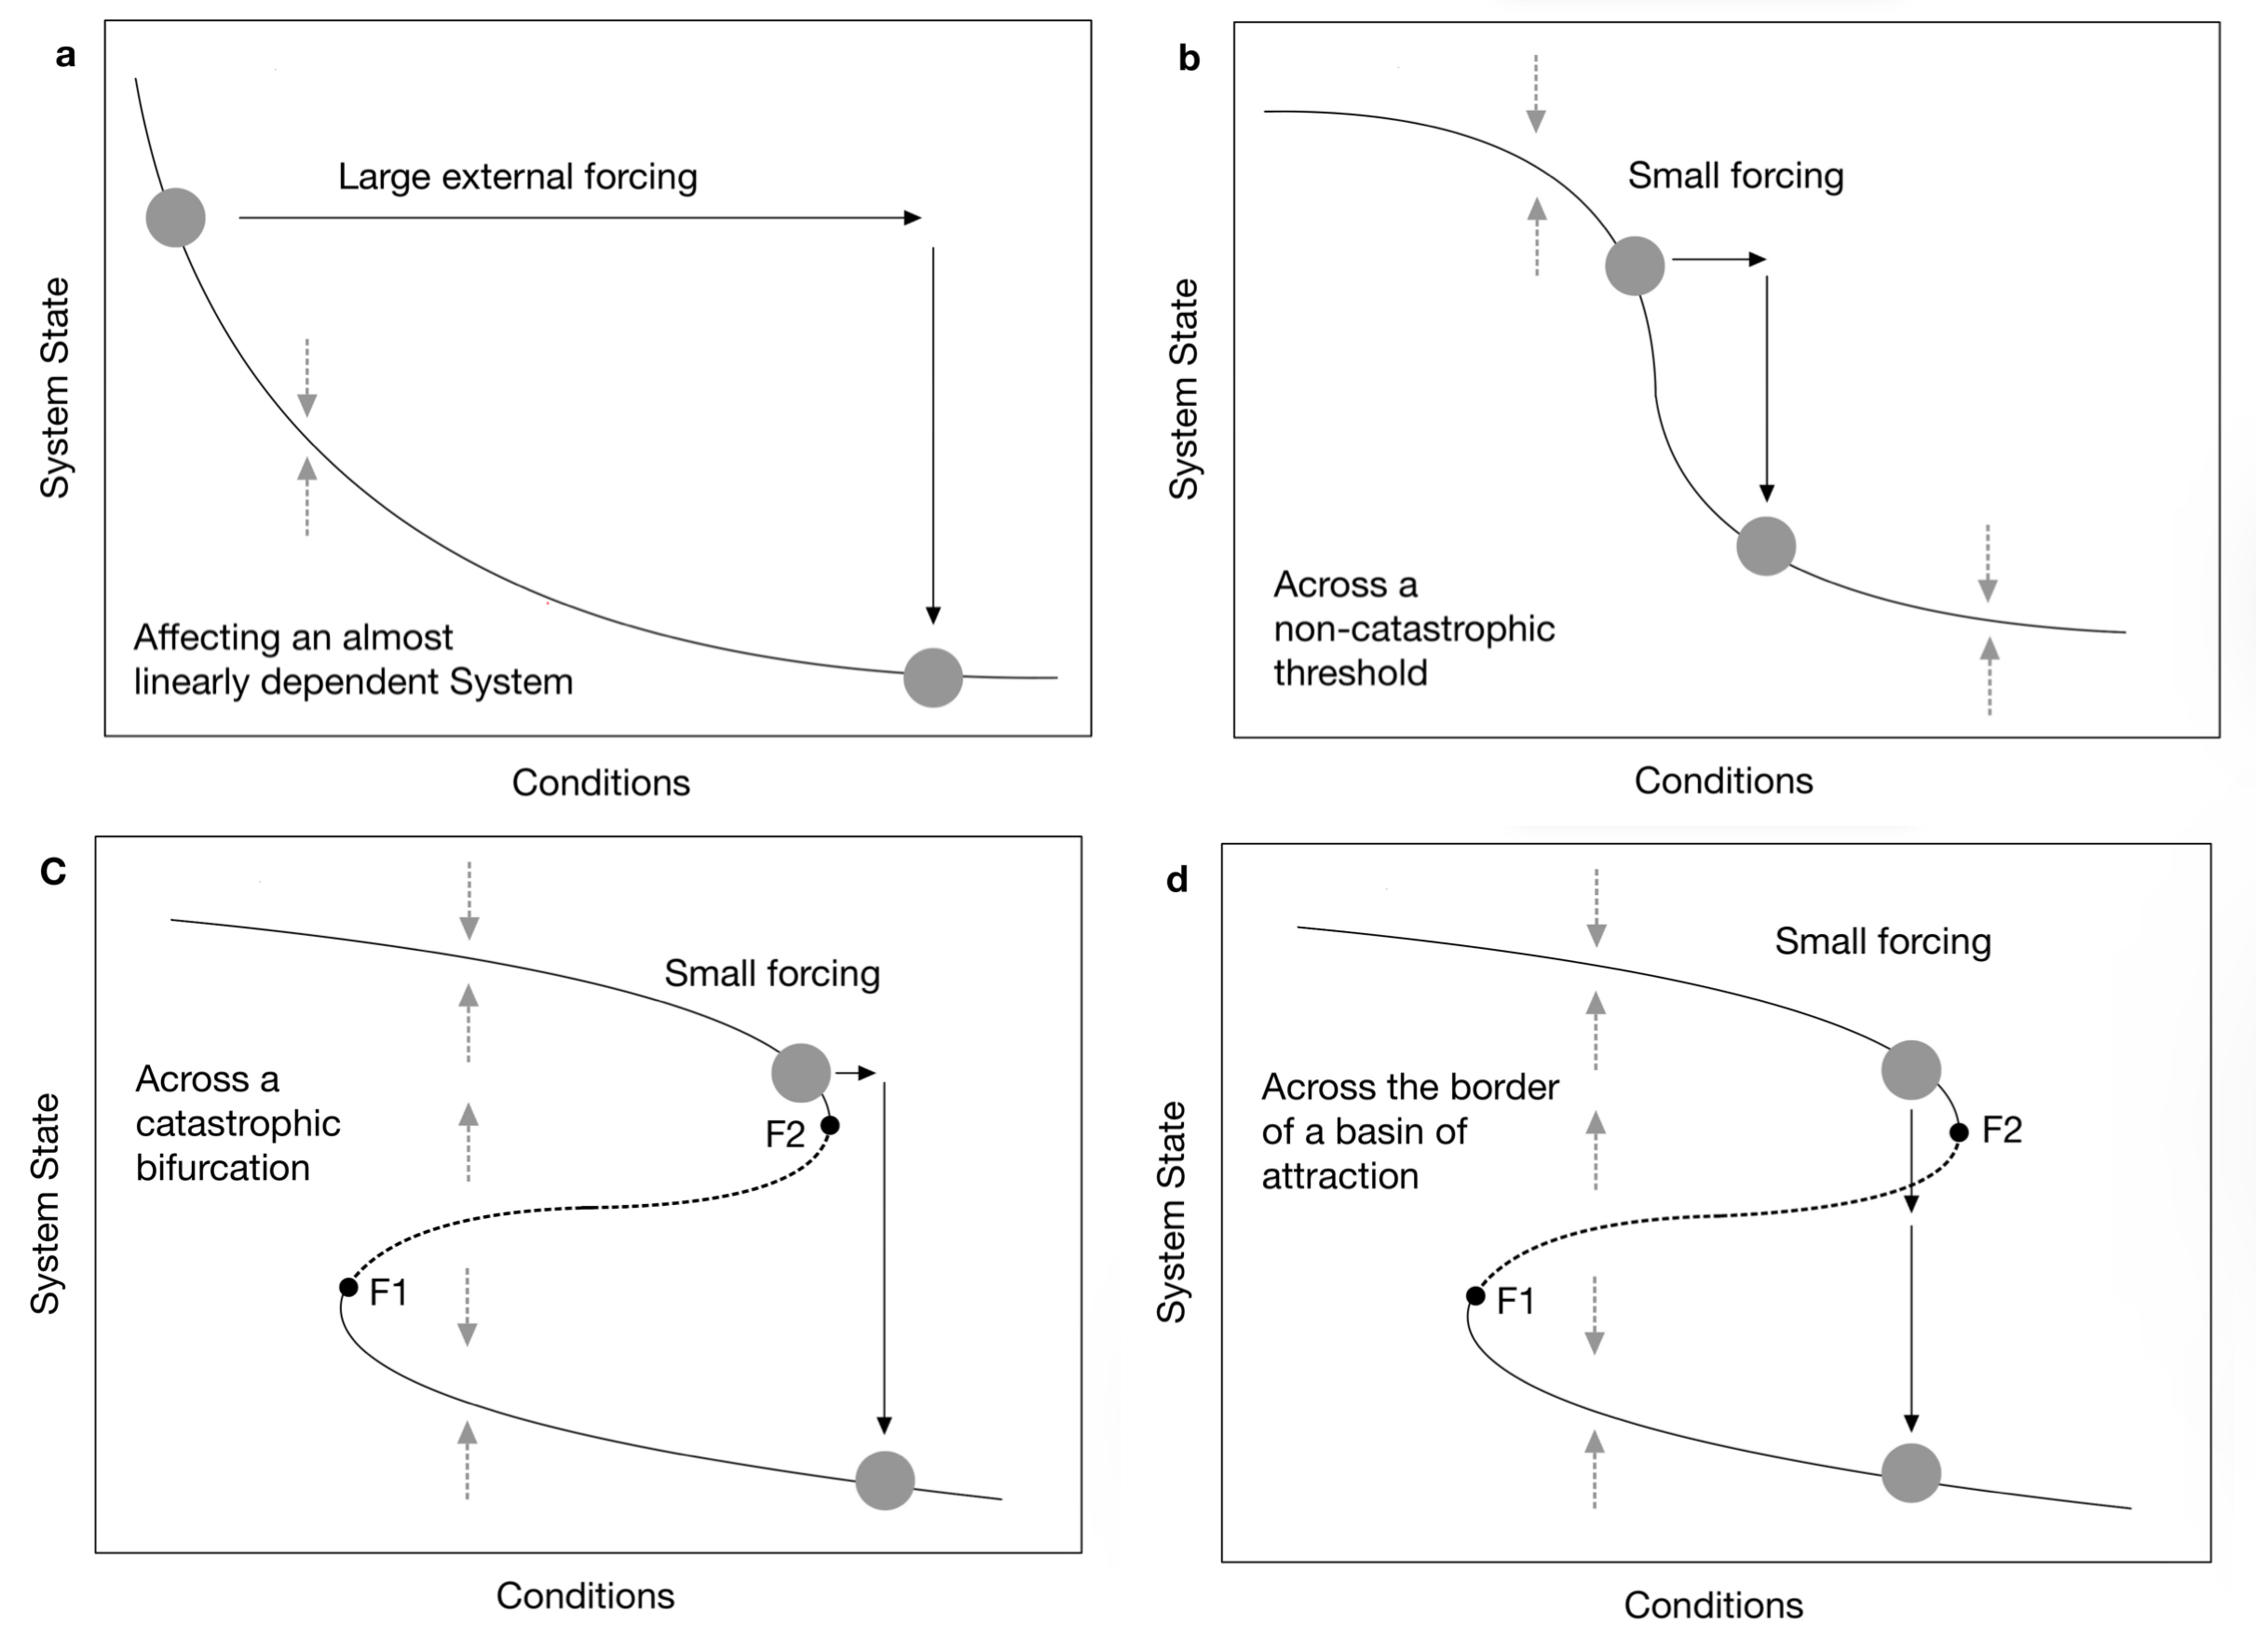
\includegraphics[width=0.8\textwidth]{bachelor-thesis/figures/scheffer_box_1.jpg}
    \caption{Based on \cite{Scheffer:2009} Box 1: Critical transitions in the fold catastrophe model. Different ways of how a dynamical system can abruptly change its system state are illustrated. In panel a the change is due to a large external forcing. Panel b shows a situation, where a small change in the conditions in a sensitive area of the system can lead to a large shift. Only in the bottom row a real bifurcation is present. The change is caused either by a small change in conditions (Panel c) or by an external forcing (Panel d).}
    \label{fig:Critical transitions in the fold catastrophe mode}
\end{figure}


\section{Motivation for the traditional EWS (TEWS): Variance and $AC(1)$}
\label{sec: Motivation for the traditional EWS: Variance and $AC(1)$}

This section mostly builds on \cite{Scheffer:2009}(paragraph: Theory).\\
The goal of early warning signals is to indicate the approaching of a tipping point in our system. Most indicators make use of the CSD phenomenon, which we want to illustrate with a simple example. The main idea behind CSD is the following: Assume we have a stochastically forced dynamical system of the form 
\begin{equation}
    \frac{dx}{dt} = f(x(t),\mu(t)) + \xi (t) 
    \label{stochastically forced system}
\end{equation}

where $\mu(t)$ is a bifurcation parameter and $\xi(t)$ is a noise term following some probability distribution for every $t \geq 0$. The system has a fold bifurcation point at $\mu_{c}$. 
We can linearize around an equilibrium $x^{*}$ (a point with $f(x^{*}(\mu),\mu) = 0$):
        \[
        f(x;\mu) \approx f(x^{*}(\mu),\mu) + \partial_{x}f(x^{*}(\mu);\mu)(x(t)-x^{*}) = \partial_{x}f(x^{*}(\mu);\mu)(x(t)-x^{*}) =: -\lambda(\mu)(x(t) - x^{*})
        \]
        
To improve legibility we omitted the time dependence of the bifurcation parameter. If the dependence of f on $\mu$ is smooth, we can expect that for $\mu \rightarrow \mu_{c}$ the recovery rate $\lambda(\mu)$ will go to zero. Hence the system will be slower in recovering from perturbations when it approaches the TP at $\mu_{c}$. This phenomenon, referred to as CSD, occurs for all continuous models approaching a fold bifurcation \cite{Wissel:1984}. Furthermore, CSD was observed in several models already far away from the bifurcation point \cite{VanNes:2007}. Now we give a simple example to illustrate the relationship between the recovery rate $\lambda(\mu)$ and proximity to a TP, following \cite{Scheffer:2009} Box 2. To do so, we consider the following system: 
\begin{equation}
    \frac{dx}{dt} = \gamma (x-a)(x-b) =: f(x) \label{eq:1}
\end{equation}
with $a,b,\gamma \in \mathbb{R}$, $a < b$ and $\gamma > 0$. The two stationary states of the system are $a$ and $b$, where $a$ is stable and $b$ is unstable. Assume $b$ is fixed and $a$ is the bifurcation parameter.
We have: 
\[\lambda (a) = -\frac{df}{dx}|_{a} = \gamma(b-a)\] 

We will now study how the system evolves if we add a small perturbation to the stable state a. Let $\epsilon(t) := x(t) - a$. We have:

\[
\frac{d\epsilon(t)}{dt} = \frac{d(a + \epsilon(t))}{dt} = f(a + \epsilon(t)) \approx 
 -\lambda(a)\epsilon(t)
\]
The solution is $\epsilon(t) = \epsilon_{0}\exp(-\lambda(a)t) = \epsilon_{0}\exp(-t/T_{R}(a))$, where $T_{R}(a) := 1/ \lambda(a)$ is the characteristic return time \cite{Wissel:1984}.
We see that for $a \nearrow b$ it holds that $\lambda(a) \searrow 0$ and $T_{R}(a)\nearrow \infty$. 
From CSD we know that the recovery rate after a small disturbance of a system is an indicator for proximity to a bifurcation point \cite{VanNes:2007}. In natural systems, it is mostly not possible to test recovery rates directly. Still, since most systems are under constant natural perturbation we can use statistics and try to deduce information about the linear recovery rate. An increase in the autocorrelation of a time series generated by equation \ref{stochastically forced system} is one important predictor for slowing down \cite{Ives:1995}. This is easy to understand intuitively: Due to the decrease in recovery rate of the system the states get more and more similar to each other. The lag-1 autocorrelation measures how closely the current state is correlated to the past state. Hence we expect an increase in this measure.

Another indicator for an approaching TP is an increase in the variance of the fluctuations of a stochastically forced system. The intuitive explanation is again simple: When the linear recovery rate goes to zero, the reverting back to the equilibrium gets very slow and the perturbations can accumulate leading to an increase in the variance. 
We will prove these properties of the TEWS methods later more formally. To do so we first introduce some concepts in the following section Prerequisites. In Figure \ref{fig:scheffer_fig_1_reimp} we give more intuition for the TEWS methods. \\



\begin{figure}[h]
    \centering
    \includegraphics[width=0.95\textwidth]{bachelor-thesis/figures/scheffer_figure1.jpg}
    \caption{Based on \cite{Scheffer:2009}, Figure 1:
    Two time series are simulated by the SDE: $dX_{t}=X(1-X/K)-c(X^2/(X^2+1))dt + dW_{t}$ modelling a harvested population with carrying capacity $K = 10$ and maximum harvest rate c (0.5 for high resilience and 2.3 for low resilience). In Panels a,b, and c the system is farther away from the TP and the recovery rate is higher. This leads to a smaller variance in the fluctuations around the equilibrium and a smaller autocorrelation. Panels d,e, and f show the system being closer to the TP with a lower recovery rate. There is a larger variance and autocorrelation.}
    \label{fig:scheffer_fig_1_reimp}
\end{figure}


\section{Structure of the Bachelor Thesis}
Following this introduction section, we will start with some theoretical prerequisites from the areas of probability theory and stochastic analysis which we will need later on. With the help of SDEs we can then define a model for stochastically forced dynamical systems and derive their stationary characteristics. This will enable us to show the potentials and shortcomings of the TEWS methods more rigorously. In the subsequent two sections we will show how to numerically integrate the SDEs for simulations of time series and provide consistent estimators for the TEWSs. Afterwards we will give the theoretical background of the ROSA indicator. Having the three EWS methods introduced we will see an example of a successful application of all indicators in a fold bifurcation setting and also the failure of the TEWS methods. A more thorough comparison of the old methods against ROSA method in terms of false positive and false negative signals follows afterwards. Finally we will apply the ROSA method to a very simple climate model.





\chapter{Prerequisites}

The areas of probability theory and stochastic analysis provide the possibility to define and analyze stochastically forced dynamical systems. We will discuss some necessary concepts from these fields in the following.

\section{Probability theory}

\begin{definition}[Stochastic process \cite{rolles:2023}]
Let I $\subseteq \mathbb{R}$. Let $X_{t}:\Omega \rightarrow \mathbb{R}, t \in I$ be a random variable on the same probability space $(\Omega,\mathcal{F},P)$. Then, $X = (X_{t})_{t \in I} $ is called a real-valued stochastic/random process. If $I = \mathbb{N}_{0}$ it is a discrete time process, if  $I = \mathbb{R}_{+}$ it is a continuous process.
\end{definition}


\begin{definition}[Gaussian process]
    A stochastic process $(X_{t})_{t\geq 0}$ is a Gaussian process if for all $t_{1} < t_{2} < ... < t_{n} \ n \in \mathbb{N}$, the vector $(X_{t_{1}},...,X_{t_{n}})$ is a Gaussian process.
\end{definition}


\begin{definition}[Autocovariance function]
Be $(X_{t})_{t \in I \subseteq \mathbb{R}}$ a random process. We define the autocovariance function: 
\[
R_{X}(t_{1},t_{2}) := Cov(X_{t_{1}},X_{t_{2}})
\]    
\end{definition}

It is called 'auto'-covariance function because the covariance is taken with respect to the same process $X_{t}$


%stanf_stat_proc
\begin{definition}[Weak sense stationarity]
A stochastic process $(X_{t})_{t\geq 0})$ is weak-sense stationary (WSS), if:

\begin{subequations}
    \begin{align}
        E[X(t)] &= \mu \ \ \forall t \geq 0 \\
        R_{X}(t_{1},t_{1} + \tau) &= R_{X}(t_{2},t_{2} + \tau) \ \ \forall t_{1},t_{2},\tau \in \mathbb{R}_{+} \\
        E[X(t)^2]&<\infty
    \end{align}
\end{subequations}   
\end{definition}

Since $R_{X}(t_{1},t_{2}) = R_{X}(t_{2},t_{1})$, $R_{X}$ is a function of $\lvert t_{2} - t_{1} \rvert$ for a WSS stochastic process and can be written as:
\[
R_{X}(\tau) := R_{X}(t,t + \tau), \ \tau \geq 0
\]

As the name suggests there is also a stronger concept of stationarity called \textit{Strong Sense Stationarity} (SSS). The latter always implies WSS, while the reverse direction isn't true in general. However, it holds for Gaussian processes (?). We will only need WSS.

Now we can also define the autocorrelation function for WSS processes:

\[
\text{AC}(\tau) := \frac{R_{X}(\tau)}{(\text{Var}(X_{t})\text{Var}(X_{t+\tau}))^{\frac{1}{2}}}, \ \tau \geq 0
\]

Later we want to compare our EWS indicators. Then we need to quantify how monotone increasing a series of values is. For this, we will use the Kendall's $\tau$ coefficient. 

\begin{definition}[Kendall's $\tau$ coefficient]
\label{def:Kendall tau}
Let $(x_{1},y_{1}),(x_{2},y_{2}),...,(x_{n},y_{n})\in \mathbb{R}^{2}$. A pair of observations $(x_{i},y_{i}),(x_{j},y_{j}), i,j \in [n]$ is concordant if it holds:
\[
((x_{i} > x_{j}) \wedge (y_{i} > y_{j})) \vee
((x_{i} < x_{j}) \wedge (y_{i} < y_{j}))
\]
Otherwise it is discordant. The Kendall $\tau$ coefficient is defined as:
\[
\tau := \frac{\#concordant\ pairs - \#number\ of\ discordant\ pairs}{\#pairs} = \frac{2}{n(n-1)}\sum_{i<j}sgn(x_{i}-x_{j})sgn(y_{i}-y_{j})
\]
where sgn is the signum function.    
\end{definition}


\section{Stochastic analysis}
\label{stochastic analysis}

\begin{definition}[Wiener process \cite{gantert:2024}]
A Wiener process is a stochastic process $(W_{t})_{t\geq 0}$ on some probability space $(\Omega,\mathcal{F},P)$ with the following properties: 
\begin{itemize}
    \item $W_{0} = 0$ P-a.s
    \item For $0 = t_{0} < t_{1} < ... < t_{n}$, the increments $W_{t_{i}} - W_{t_{i-1}}, 1 \leq i \leq n$, are independent with law $N(0,t_{i}-t_{i-1})$
    \item $t \mapsto W_{t}(\omega)$ is continuous for P-a.a $\omega \in \Omega$
\end{itemize}
\end{definition}

Interpretation: 

\begin{itemize}
    \item $\forall \ t \geq 0, \ W_{t}: \Omega \mapsto \mathbb{R}$ is a random variable 
    \item $(W_{t})_{t \geq 0} : \Omega \mapsto C[0,1]$ is a random variable that takes an $\omega$ as input and outputs one realization of a path
\end{itemize}

We define the \textit{Cameron-Martin-Space} as:
\[
H_{t} := \{ h \in C[0,t]: \exists f \in L^{2}[0,t] \ s.t \  h(s) = \int_{0}^{s} f(\tau) d\tau, 0 \leq s \leq t \}
\]

For $h \in H_{t},\ f \in L^{2}[0,t]$ is uniquely determined and we write: 
\[
h' = f
\]
(In genereal $h$ does not have to be differentiable for every $s \in [0,t]$)

Now we can define stochastic integrals for a certain class of functions:

\begin{lemma}[The Paley-Wiener stochastic integral \cite{gantert:2024}] 
Let $(W_{s})_{s\geq 0}$ be a Wiener process and $h \in H_{t}, t \geq 0$. Then:
\[
\xi_{n}^{t} := 2^{n}\sum_{j=1}^{2^{n}}(h(\frac{tj}{2^{n}})-h(\frac{t(j-1)}{2^{n}}))(W_{\frac{tj}{2^{n}}}-W_{\frac{t(j-1)}{2^{n}}}) 
\]

converges P-a.s and in $L^{2}$. We denote the limit of n to infinity by
\[
\int_{0}^{t}h'(s)dW_{s} = \int_{0}^{t}h'dW
\]
\end{lemma}

At this point we want to highlight the importance of the fact that in the definition of the Wiener process the variance of $W_{t}$ is defined to be proportionate to time. Per definition it holds $W_{t} \sim N(0,t)$. Suppose we choose a power $t^{\alpha}, \alpha > 0$ for the variance of $W_{t}$. 

With $h(s) := s, \ s \in [0,t]$ it holds $h \in H_{t}$ and $h' \equiv 1$. Further we have: $\int_{0}^{t} 1 dW_{s} = W_{t} = \xi_{n}^{t}, \ \forall n \in \mathbb{N}$ and $Var[W_{t}] = t^{\alpha}$ by assumption. From 
$t^{\alpha} = Var[\xi_{n}^{t}] = Var\left[\sum_{j=1}^{2^{n}}\left(W_{\frac{tj}{2^{n}}} - W_{\frac{t(j-1)}{2^{n}}}\right)\right] = 2^{n}Var\left[W_{\frac{t}{2^n}}\right] = 2^{n}\left(\frac{t}{2^{n}}\right)^{\alpha}, \ \forall n \in \mathbb{N}$ it follows that $\alpha$ has to equal 1, where we used that the increments are independent and identically distributed (i.i.d.)  \\

Consider the process:

\begin{definition}[Ornstein-Uhlenbeck process (SA script Example 10.7)] 
For $\alpha > 0$, $(W_{t})_{t\geq 0}$ a Wiener process, $x_{0} \in \mathbb{R}$. Consider the following SDE:
\[
dU_{t} = -\lambda U_{t} dt + \sigma dW_{t}, U_{0} = u_{0}
\]
\label{def:OU process}
or equivalently
\[
U_{t} = u_{0} - \lambda\int_{0}^{t}U_{s}ds + \sigma W_{t}, t \geq 0
\]  
\end{definition}

$\textbf{Claim}$: 
\[
U_{t} = \exp(-\lambda t)u_{0} + \sigma\int_{0}^{t}\exp(-\lambda (t-s))dW_{s}
\]
solves the above SDE. We check this applying Ito's product rule to $\sigma e^{-\lambda t}\int_{0}^{t}e^{\lambda s}dW_{s}$:
\[
dU_{t} = -\lambda u_{0}e^{-\lambda t}dt - \lambda\sigma(e^{-\lambda t}\int_{0}^{t}e^{\lambda s}dW_{s})dt + \sigma e^{-\lambda t}e^{\lambda t}dW_{t} = -\lambda U_{t} dt + \sigma dW_{t}
\]

If we choose $U_{0} \sim N(0,\frac{\sigma^{2}}{2\lambda})$ as an initial distribution, which is independent of $(W_{t})_{t\geq 0}$ than $E[U_{t}] = 0$, $Cov[U_{s},U_{t}] = \frac{\sigma^2}{2\lambda}e^{(-\lambda\lvert t-s \rvert)}$ for $t,s \geq 0$ and $U_{t}$ is wide sense stationary. It follows that $Var[U_{t}]=E[(U_{t})^{2}]=\frac{\sigma^2}{2\lambda}$ and $U_{t} \sim N(0,\frac{\sigma^2}{2\lambda}), \forall t \geq 0$ because the sum of normal random variables is again a normal random variable.

To prove the statements about the expectation and the covariance of $U_{t}$ we use some results from stochastic analysis and probability theory.
From stochastic analysis we use a weaker form of Ito's isometry:

%use abs value
\begin{lemma}[Ito's isometry]
 Let $t \geq 0$ and $g \in L^2[0,t]$. Then:
 \[
 E[(\int_{0}^{t}g(s)dW_{s})^{2}] = \int_{0}^{t}g(s)^2ds
 \]
\end{lemma}

The following Lemma shows that $\int_{0}^{t}e^{\alpha s}dW_{s}$ is a martingale.   \textit{(I)}

\begin{lemma}
    Let $g \in L^2[0,t]$ for every $t \geq 0$. Then $(\int_{0}^{t}g(s)dW_{s})_{t\geq 0}$ is a martingale and hence:
    \[
    E[\int_{0}^{t}g(s)dB_{s}] = 0, \ \forall t \geq 0
    \]
\end{lemma}

From probability theory we use the following two results about conditional expectations:

\begin{lemma}
    Let $X: \Omega \rightarrow \mathbb{R}$ be an $(\mathcal{F}_{0},\mathcal{B}(\mathbb{R}))$- measurable random variable with $E[\lvert X \rvert] < \infty$ or $X \geq 0$ and $\mathcal{F} \subseteq \mathcal{F}_{0}$ a $\sigma$-algebra. Then it holds:
    \[
    E[E[X|\mathcal{F}]] = E[X]
    \]
\end{lemma}

\begin{lemma}
    If X is $\mathcal{F}$-measurable, $E[\lvert XY \rvert] < \infty$ and $E[\lvert Y \rvert]< \infty$ then:
    \[
    E[XY|\mathcal{F}] = XE[Y|\mathcal{F}], \ P-a.s
    \]
\end{lemma}

Let $0 \leq s \leq t$. Then:

\[
E[U_{t}] = e^{-\lambda t}E[U_{0}] + e^{-\lambda t}E[\int_{0}^{t} e^{\lambda s} dW_{s}] = e^{-\lambda t}E[\int_{0}^{t} e^{\lambda s} dW_{s}] \stackrel{(I)}{=}  0
\]

Next we want to prove: $Cov[U_{s},U_{t}] = \frac{1}{2\lambda}e^{-\lambda \lvert t-s \rvert}$. 
\begin{equation}
    Cov[U_{s}U_{t}]=E[U_{s}U_{t}] = e^{-\lambda(t+s)}E[U_{0}^{2}] + \sigma^2 e^{-\lambda(t+s)}E[\int_{0}^{t}e^{\lambda u}dW_{u}\int_{0}^{s}e^{\lambda v}dW_{v}]
    \label{cov white noise noise}
\end{equation}

We show that for any martingale $(M_{t})_{t \geq 0}$ the following holds: 
\begin{equation}
    E[M_{t}M_{s}] = E[M_{s}^{2}], \ s \leq t
    \label{result cond exp}
\end{equation}

Lemma 5 gives us:
\[
E[M_{t}M_{s}] = E[E[M_{t}M_{s}|\mathcal{F}_{s}]]
\]
Since $M_{s}$ is $\mathcal{F}_{s}$-measurable, Lemma 6 yields:
\[
E[E[M_{t}M_{s}|\mathcal{F}_{s}]] = E[M_{s}E[M_{t}|\mathcal{F}_{s}]]
\]
For a martingale it holds: $E[M_{t}|\mathcal{F}_{s}] = M_{s}, s \leq t$. Equation \ref{result cond exp} follows. Continue with \ref{cov white noise noise}:


\begin{subequations}
    \begin{align*}
        E[U_{s}U_{t}] &= \frac{\sigma^2}{2\lambda}e^{-\lambda(t+s)} + \sigma^2 e^{-\lambda(t+s)}E[(\int_{0}^{s}e^{\lambda v}dW_{v})^{2}]   \\
         &= \frac{\sigma^2}{2\lambda}e^{-\lambda(t+s)} + \sigma^2 e^{-\lambda(t+s)}\int_{0}^{s}e^{2\lambda v}dv, \ \ \ (Lemma \ 2) \\
         &= \frac{\sigma^2}{2\lambda}e^{-\lambda(t+s)} + e^{-\lambda(t+s)}\frac{\sigma^2}{2\lambda}(e^{2\lambda s} - 1) \\
         &= \frac{\sigma^2}{2\lambda}e^{-\lambda(t-s)} 
    \end{align*}
\end{subequations}   

\qed

Hence it holds for $\tau > 0$:
\[
R_{X}(\tau) =  \frac{\sigma^2}{2\lambda}\exp(-\lambda\tau)
\]


\section{Continuous time stochastic modeling}
\label{Continuous time stochastic modeling}
From \cite{Morr:2022}.

We want to motivate the use of certain stochastic differential equations, which we will use later. 
In dynamical modeling it is common to describe the system of interest with a deterministic forcing plus a noise term to capture the unresolved dynamics. We can construct a discrete-time stochastic process following this approach:

\begin{equation}
    X_{k+1}-X_{k} = f(X_{k},k) + \sigma\epsilon_{k}, X_{0} = x_{0} \in \mathbb{R}
    \label{eq:discrete-time modelling}
\end{equation}

A usual choice for the noise term would be independent $\epsilon_{k} \sim \mathcal{N}(0,1)$, also called Wiener or white noise \cite{zwanzig:2001}.
Yet in some applications the assumption of independence of the stochastic increments may be unsuitable due to memory effects in the unresolved dynamics \cite{zwanzig:1961,chorin:2000}.

One common way to model correlated noise is via an AR(1)-process:
\[
\epsilon_{k+1} = \phi\epsilon_{k} + z_{k}, \epsilon_{0} \sim \mathcal{N}(0,(1-\phi^2)^{-1})
\]
with $0<\phi<1$ and $(z_{k})_{k}\in\mathbb{N}$ i.i.d standard Normal random variables. This type of noise is also called \textit{red noise}. With the specific choice of the distribution of $\epsilon_{0}$ the process is weakly stationary. We prove this only considering $\tau = 1$ for the autocorrelation function, since later we are only interested in $R_{X}(1)$. First we show by induction that: $\epsilon_{k} \sim \mathcal{N}(0,(1-\phi^2)^{-1}), \forall k \in \mathbb{N}_{0}$. Since $\epsilon_{k}$ is a normal random variable $\forall \ k \in \mathbb{N}_{0}$ it is enough to prove the statements for the expectation and variance. The statements hold for $\epsilon_{0}$ by definition. Suppose the statements hold for $k \in \mathbb{N}$. Then:

\begin{subequations}
    \begin{align}
        E[\epsilon_{k+1}] &= \phi E[\epsilon_{k}] + E[z_{k}]  = 0 \\
        Var[\epsilon_{k+1}] &= \phi^2 Var[\epsilon_{k}] + 1 = \frac{\phi^2}{1-\phi^2} + 1 = \frac{1}{1-\phi^2}     
    \end{align}
\end{subequations}   

by the linearity of the expectation, properties of the variance, the induction hypothesis, the fact that $z_{k} \sim \mathcal{N}(0,1) \ \forall k \in \mathbb{N}_{0}$ and the independence of $\epsilon_{k}$ and $z_{k}$. Now to show that $R_{\epsilon}(k,k+1) = R_{\epsilon}(0,1) \forall k \in \mathbb{N}_{0}$ it suffices to show that $Cov[\epsilon_{k},\epsilon_{k+1}] = E[\epsilon_{k}\epsilon_{k+1}] - E[\epsilon_{k}]E[\epsilon_{k+1}] = E[\epsilon_{k}\epsilon_{k+1}] = E[\epsilon_{0}\epsilon_{1}] \forall \ k \in \mathbb{N}_{0}$. This follows from: 
\[
E[\epsilon_{k}\epsilon_{k+1}] = E[\epsilon_{k}(\phi\epsilon_{k} + z_{k})] = \phi E[\epsilon_{k}^2] = \phi E[\epsilon_{0}^2] = E[\epsilon_{0}\epsilon_{1}]
\]

The $(\epsilon_{k})_{k \in \mathbb{N}}$-process has an exponentially decaying correlation structure. \textbf{Claim}:
\[
R_{\epsilon}(\tau) = \frac{\phi^{\tau}}{1-\phi^{2}}, \tau \in \mathbb{N}_{0}
\]
\textbf{Proof}: \\
It holds: 
\[
R_{\epsilon}(0)= Var(\epsilon_{k}) = \frac{1}{1-\phi^{2}}
\]
Further it holds for $\tau, k \in \mathbb{N}_{0}$:
\[
R_{\epsilon}(\tau+1) = Cov[\epsilon_{k},\epsilon_{k+\tau + 1}] = Cov[\epsilon_{k},\phi\epsilon_{k+\tau}+z_{k+\tau}] = \phi R_{\epsilon}(\tau)
\]
since $\epsilon_{k}$ and $z_{k+\tau}$ are independent. Hence for $\tau \in \mathbb{N}_{0}$:
\[
R_{\epsilon}(\tau) = \phi^{\tau}R_{\epsilon}(0)=\frac{\phi^{\tau}}{1-\phi^{2}}
\]
\qed

The use of continuous models is often advantageous when describing systems in nature. With the help of stochastic analysis, we can include randomness into these models. In a similar way to equation \ref{eq:discrete-time modelling} we can use: 

\begin{equation}
    dX_{t} = f(X_{t},t)dt + \sigma dY_{t}, X_{0} = x_{0} \in \mathbb{R}
    \label{eq:continuous time modelling}
\end{equation}

Traditionally the Wiener process $Y = W = (W_{t})_{t\in \mathbb{R}_{+}}$ is used for uncorrelated noise. The notation in \ref{eq:continuous time modelling} is just a shorthand for the following integral equation:
\[
X_{t} = X_{0} + \int_{0}^{t}f(X_{s},s)ds + \sigma Y_{t}
\]

where $Y_{t}$ is in the class of Ito-processes that have the following form:
\begin{equation}
    Y_{t} = Y_{0} + \int_{0}^{t}\alpha_{s}ds + \int_{0}^{t}\beta_{s}dW_{s}
    \label{eq:Ito process}
\end{equation}

with $\alpha = (\alpha_{t})_{t\in\mathbb{R}_{+}}$ and $\beta = (\beta{t})_{t\in\mathbb{R}_{+}}$ being suitable processes.
In \cite{Morr:2022} Morr et al. want to translate the concept of correlated noise from discrete-time models to the continuous case. As we will see, when discussing how to simulate SDEs, the Euler-Mayurama method enables us to translate the continuous case into a discrete one. The opposite task is not uniquely determined. However under certain assumptions the number of possible processes for $Y_{t}$ can be reduced. First, we assume that $Y_{t}$ has the form $\alpha_{t}dt$. Since $(\epsilon_{k})_{k\in\mathbb{N}_{0}}$ is a discrete-time stationary Gaussian Markov process, we also require $\alpha = (\alpha_{t})_{t\in\mathbb{R}_{+}}$ to have these properties in continuous time. According to \cite{doob:1942} all measurable, stationary, Gaussian, Markov processes are of the Ornstein-Uhlenbeck type. (argument to narrow, scaling autocov?).

However, we didn't justify the prehand restriction to $dY_{t} = \alpha dt$. We will now turn to spectral characteristics of the $(\epsilon_{k})_{k\in\mathbb{N}_{0}}$ process to motivate this constraint. One important characteristic of a stochastic process is its Power Spectral Density:


\begin{definition}[Power Spectral Density (PSD)]
The PSD of a stochastic process $(X_{t})_{t \geq 0}$ is given by:
\[
S_{X}(\omega) := lim_{T\rightarrow\infty}E[\lvert \frac{1}{\sqrt{T}}\int_{0}^{T}\exp(-i\omega t)X_{t}dt\rvert^{2}], \ \omega \in \mathbb{R}
\]
if the limit exists.
\end{definition}

\begin{theorem}[Wiener-Khinchin theorem]
Let $(X_{t})_{t}$ be a (wide sense) stationary, centered process with $E[X_{t}^2]<\infty \ \forall t \geq 0$ and absolutely integrable $R_{x}(\tau)$. Then we have:
\[
S_{X}(\omega) = \mathcal{F}[R_{X}(\tau)](\omega) := \int_{-\infty}^{\infty}\exp(-i\omega\tau)R_{X}(\tau)d\tau
\]
\end{theorem}

Equivalent results hold for discrete processes, replacing the integrals by Riemann sums.

We require our process $Y_{t}$ to have the same PSD as its discrete counterpart $\epsilon_{k}$, which we can calculate via the discrete Wiener-Khinchin theorem:
\[
S_{\epsilon} = \mathcal{F}[R_{\epsilon}(\tau)](\omega) = \frac{-2log(\phi)}{(1-\phi^{2})(log(\phi)^{2}+\omega^{2})} = \mathcal{O}(\omega^{-2})
\]

In many applied areas the decay rate of $\mathcal{O}(\omega^{-2})$ is the defining property of red noise. Indeed the term \textit{red noise} is due to the fact that low frequencies have the highest amplitude in red light and the PSD. 
Under appropriate technical assumptions on $\alpha$ and $\beta$ used in \ref{eq:Ito process}, demanding a vanishing PSD of $Y_{t}$ in the high-frequency domain implies $\beta_{t} = 0$ P-a.s $\forall t \geq 0$, justifying the previous restriction. Together with the reasoning about Gaussian Markov processes from above, we get that the Ornstein-Uhlenbeck process $U_{t}$, with initial distribution $X_{0} \sim \mathcal{N}(0,(1-\phi)^2)$ is a unique way to model continuous time red noise. Hence we choose $dY_{t} = \alpha_{t}dt = U_{t}dt$. 

Both the exponential decay of the autocovariance function and the characteristic decay rate of $\mathcal{O}(\omega^{-2})$ for the PSD is shown by the Ornstein-Uhlenbeck process $U_{t}$, as we have seen for the discrete-time red noise process $(\epsilon_{k})_{k\in\mathbb{N}_{0}}$. We already calculated $R_{U}(\tau)$. 
An application of the Wiener-Khinchin theorem gives us: 
\[
    S_{U}(\omega) = \frac{1}{\theta^{2} + \omega^{2}}
\]
We complete the Prerequisites section by motivating the term 'white' noise for Wiener noise. The PSD of $W_{t}$ is constant:
\[
S_{W}(\omega) =  lim_{T\rightarrow\infty}E[\frac{1}{T}\lvert\int_{0}^{T}\exp(-i\omega t)dW_{t}\rvert^{2}] = lim_{T\rightarrow \infty}E[\frac{1}{T}\int_{0}^{T}1dt] = 1
\]
where Ito's isometry was used in the second equality.



\chapter{SDE settings and their stationary characteristics}

We already motivated the use of stochastically forced dynamical systems described by an SDE of the form:
\begin{equation}
    dX_{t} = f(X_{t},t)dt + \sigma dY_{t}, X_{0} = x_{0} \in \mathbb{R}
    \label{eq:SDE for stochastically forced dynamical systems}
\end{equation}
With this, we want to capture the dynamics of a fold bifurcation system (in our case e.g. an earth system component that exhibits a TP) driven by a bifurcation parameter $\mu(t)$ with unresolved dynamics being included in the noise term. Our main interest is in the linearized dynamics of the system around an equilibrium path $X^{*}(\mu)$ and we would like to gain information about the evolution of the linear recovery rate $\lambda(\mu)$. In the case of CSD we have $\lambda(\mu) \searrow 0$ and this gives us the possibility of an EWS before reaching a tipping point. The use of the traditional EWS $AC(1)$ and Variance has been motivated intuitively. Shortly we mentioned that these two indicators lack reliability in terms of false positives or false negative signals due to their stationarity assumption on the system. This motivates the introduction of the more robust ROSA method. 
In the following, we will introduce two SDE settings for the linearized dynamics of equation \ref{eq:SDE for stochastically forced dynamical systems}. 
After deriving the stationary characteristics of these SDE's we can justify the use of the old EWS more rigorously. Both settings will also be used to test and compare the old methods against the new one.
One way to model the linearized dynamics around an equilibrium $X^{*}(\mu)$ is via white noise $W_{t}$:
\begin{equation}
        dX_{t}^{(w)} = -\lambda X_{t}^{(w)}dt + \sigma dW_{t}, X_{0}^{(w)} = 0, \ \ \lambda,\sigma \in \mathbb{R}
        \label{eq: white noise linearized SDE}
\end{equation}
This is an Ornstein-Uhlenbeck process, which we already introduced in the section Prerequisites. Why could it make sense to model our unresolved dynamics with Gaussian noise? This is due to the Central Limit Theorem, which states that for $X_{i}, i \geq 0$ i.i.d. random variables with finite variance the standardization of their sum converges in distribution to a standard normal random variable. Hence in the limit, this sum has a Gaussian probability density. When we model a physical system like some earth-system component with a SDE that undergoes a bifurcation, than we have processes on different time scales. The bifurcation 'lives' on a much slower time scale than the unresolved dynamics realized by the noise term. The increment $dY_{t}$ is the sum of many smaller events. If we assume that we can treat these different events as i.i.d random variables then the total impact $dY_{t}$ would be the sum of the smaller impacts and would follow a normal distribution such as $dW_{t} \sim N(0,dt)$. \cite{Kurt:2010} \\
The increments $dW_{t}$ are independent. However, as explained in the last section, this assumption is often violated in nature. We can represent memory in the system by using the following linearized red noise model \cite{Hanggi:1994,Morr:2022}:

\begin{subequations}
    \begin{align}
        dX_{t} &= -\lambda X_{t}dt + \kappa U_{t}dt, X_{0} = 0 \label{eq: 3.2a} \ \ \lambda,\kappa \in \mathbb{R}  \\ 
        dU_{t} &= -\theta U_{t}dt + dW_{t}, U_{0} = 0 \label{eq: 3.2b} \ \ \theta \in \mathbb{R}
    \end{align}
    \label{eq:red noise linearized SDE}
\end{subequations}

Here the term $\kappa U_{t}dt$ is itself described by an OU-process and the parameter $\theta$ controls the memory of the noise. There also exist other positive correlated continuous models, but the frequency properties of red noise are the best suited for many applications in Physics including the climate system \cite{Hasselmann:1976, Hanggi:1993, Liao:2022}. 
Now we want to explicitly solve the SDEs for $X_{t}^{(w)}$ and $X_{t}$. We already solved \eqref{eq: white noise linearized SDE} in the section prerequisites. To solve \eqref{eq:red noise linearized SDE} we can treat $U_{t}$ and $X_{t}$ for a moment as deterministic functions of time and use the variations of constants formula for ODE's (Appendix Math Bio): \\

\begin{lemma}[Variations of constants]
    Let $I \subset \mathbb{R}$ be an open interval. The initial value problem
        
    \begin{subequations}
        \begin{align}
            \dot{y}(t) &= a(t)y(t) + b(t)  \\
            y(t_{0}) &= y_{0}
        \end{align}
    \end{subequations}
    with $a,b : I \mapsto \mathbb{R}$ continuous has a unique solution on $I$ given by:
    \[
    y(t) = y_{0}e^{A(t)} + \int_{t_{0}}^{t}e^{A(t)-A(s)}b(s)ds, \ \ \ \ \ where \ A(t) = \int_{t_{0}}^{t}a(s)ds
    \]
\end{lemma}
In our case we have $a(t) \equiv -\lambda$ and $b(t) = \kappa U_{t}$. Hence the solution for $X_{t}$ is given by:

\begin{equation}
    X_{t} = \kappa\int_{0}^{t}\exp(-\lambda(t-s))U_{s}ds
    \label{red noise solution}
\end{equation}

The next step is to derive the stationary characteristics, namely AC(1) and Variance, for both processes. We will also compute the PSD for the theoretical background of the ROSA method, discussed in section 6. Consistent estimators for the stationary characteristics will be provided. These can than be applied to a time series generated by the SDEs introduced above or to paleoclimate records. 

For the ROSA method we will be interested in retrieving $\lambda$ by fitting to the PSD. We already showed that the OU-process $X_{t}^{(w)}$ is wide-sense stationary $\forall t \geq 0$ using $X_{0}^{(w)} \sim N(0,\frac{\sigma^2}{2\lambda})$ as an initial distribution. Additionally, we computed its characteristics. See a summary in table \ref{tab:white_noise_stat_char}. 


\begin{table}[t]
\centering
\begin{tabular}{|c|c|}
\hline
& stationary characteristics\\
\hline
Variance & $\sigma^2$ / $(2\lambda)$\\
AC($\tau$) & $\exp(-\lambda |\tau|)$\\
c.t PSD $S(\omega)$ & $\sigma^2$/($\lambda^2 + \omega^2$)\\
\hline
\end{tabular}
\caption{stationary characteristics of $X_{t}^{(w)}$}
\label{tab:white_noise_stat_char}
\end{table}

Suppose we chose $X_{0}^{(w)} = 0$ as an initial distribution instead. We will show that $X_{t}^{(w)}$ is asymptotically stationary. We can perform the same calculations as in section (\ref{stochastic analysis}) with the different initial distribution to get:

 \begin{align*}
    E(X_{t}^{(w)}) &= 0   && \forall t \geq 0 \\
    \text{Cov}(X_{t}^{(w)},X_{s}^{(w)}) &= \frac{\sigma ^2}{2\lambda}(e^{-\lambda\lvert t-s \rvert}-e^{-\lambda(t+s)}) && \forall t, s \geq 0 \\
    \text{Var}(X_{t}^{(w)}) &= \frac{\sigma^2}{2\lambda}(1-\exp(-2\lambda t)) && \forall t \geq 0 
\end{align*}

For $t\rightarrow \infty$ it follows: 
\[
\text{Var}(X_{t}^{(w)})\rightarrow\frac{\sigma^2}{2\lambda}
\]
and 
\[
\text{Cov}(X_{t}^{(w)},X_{t+\tau}^{(w)}) = \frac{\sigma^2}{2\lambda}(e^{-\lambda\lvert \tau \rvert} - e^{-\lambda(2t + \tau)}) \rightarrow \frac{\sigma ^2}{2\lambda}\exp(-\lambda\lvert \tau \rvert) = R_{X^{(w)}}(\tau)
\]
Hence we see that in the limit $t\rightarrow \infty$, $X_{t}^{(w)}$ converges to the same stationary distribution as for the case $X_{0}^{(w)} \sim N(0,\frac{1}{2\lambda})$. 
In applications, we take the stationary characteristics as good approximations also for finite times.

Now we turn to the red noise case. We can again either have $X_{0} = 0, U_{0} = 0$ and get a stationary distribution in the limit or we use a certain initial distribution $(X_{0},U_{0})$ such that $X_{t}$ is stationary for all $t \geq 0$. The stationary characteristics of the red noise case are provided in table \ref{tab:red_noise_stat_char}.

\begin{table}[h!]
\centering
\begin{tabular}{|c|c|}
\hline
& stationary characteristics\\
\hline
Variance & $\kappa^2$ / $(2\lambda\theta(\lambda + \theta))$\\
AC($\tau$) & $(\lambda\exp(-\theta\lvert\tau\rvert)-\theta\exp(-\lambda\lvert\tau\rvert))/(\lambda - \theta)$\\
c.t PSD $S(\omega)$ & $\kappa^2/((\theta^2 + \omega^2)(\lambda^2 + \omega^2))$\\
\hline
\end{tabular}
\caption{stationary characteristics of $X_{t}$ with $\lambda \neq \theta$. The case $\lambda = \theta$ coincides with the limit $\theta \rightarrow \lambda$ for the case $\lambda \neq \theta$.}
\label{tab:red_noise_stat_char}
\end{table}

We derive these properties. As we have seen already the OU process is a Gaussian process. Since the Riemann sums of normal random variables converge again to a normal random variable it follows that also $X_{t}$ is a Gaussian process. We write \eqref{eq:red noise linearized SDE} more compact as a linear system of SDEs: 
\[
dY_{t} = AY_{t}dt + BdW_{t}
\]
where:
\[
Y_{t} = 
\begin{pmatrix}
   X_{t} \\
   U_{t}
\end{pmatrix}
,\ A = 
\begin{pmatrix}
    -\lambda &  \kappa \\
    0        & -\theta
\end{pmatrix}
,\ B = 
\begin{pmatrix}
    0 & 0 \\
    0 & 1
\end{pmatrix}
\]

\begin{align*}
V:&=\Exp{\left(X_t,Y_t\right)^\top\left(X_t,Y_t\right)}\\&=\Exp{\int_0^t\int_0^t\exp((t-s_1)A)\Sigma\begin{pmatrix}\dint W_{s_1}^{(1)}\\\dint W_{s_1}^{(2)}\end{pmatrix}\left(\dint W_{s_2}^{(1)},\dint W_{s_2}^{(2)}\right)\Sigma^\top\exp((t-s_2)A)^\top}\\
&=\int_0^t\exp((t-s)A)\Sigma\Sigma^\top\exp((t-s)A)^\top\dint s
\end{align*}

\begin{equation*}
R(\tau):=\Exp{\left(X_t,Y_t\right)^\top\left(X_{t+\tau},Y_{t+\tau}\right)}=\exp(\tau A)V.
\end{equation*}


Given that $X_{t}$ and $U_{t}$ are Gaussian processes it holds: $Y_{t} \sim N(\mu(t),\Sigma(t)),\ \mu(t) \in \mathbb{R}^{2}, \ \Sigma(t) \in \mathbb{R}^{2x2}, \ \forall t\geq 0$. We want to find a $\Sigma_{0} \in \mathbb{R}^{2x2}$ for $(X_{0},U_{0}) \sim N(0,\Sigma_{0})$ such that $\Sigma(t) \equiv \Sigma_{0}$. We can do this by solving the following Lyapunov equation corresponding to the linear system of SDEs above \cite{gardiner:2009}: 
\[
0 = \dot{\Sigma}(t) = A\Sigma(t) + \Sigma(t) A^{T} + BB^{T} 
\]
The solution is given by: 
\[
\Sigma_{0} = 
\begin{pmatrix}
    \frac{\kappa^{2}}{2\lambda\theta(\lambda + \theta)} & \frac{\kappa}{2\theta(\lambda + \theta)} \\
    \frac{\kappa}{2\theta(\lambda + \theta)} & \frac{1}{2\theta}
\end{pmatrix}
\]
We get the autocovariance function $R_{X}(\tau)$ by computing the first entry of: 
\[
E[(X_{t+\tau},U_{t+\tau})^{T}(X_{t},U_{t})] = \kappa^{2}\frac{\lambda\exp(-\theta\lvert\tau\rvert)-\theta\exp(-\lambda\lvert\tau\rvert)}{2\lambda\tau(\lambda^{2}-\theta^{2})} = R_{X}(\tau)
\]
and the PSD by an application of the Wiener-Khinchin theorem:
\[
S_{X}(\omega) = \mathcal{F}[R_{X}(\tau)](\omega) = \frac{\kappa^{2}}{(\theta^{2} + \omega^{2})(\lambda^{2} + \omega^{2})}
\]

Letting $\kappa \rightarrow \infty, \theta \rightarrow \infty, \frac{\kappa}{\theta} \rightarrow \sigma$ we observe that the characteristics of $X_{t}^{(w)}$ are a parameter limit of the characteristics of $X_{t}$. This is why we will consider only $X_{t}$ in sections 5, 8, and 9.
Another important observation is the symmetry of the stationary characteristics of $X_{t}$ with respect to a swap of $\lambda$ and $\theta$. Hence we have to be careful when we want to infer e.g. information about $\lambda$.

\begin{table}[h!]
\centering
\begin{tabular}{|c|c|c|c|}
\hline
& Variance & AC(1)\\
\hline
$\lambda \rightarrow 0$ & $\nearrow \infty$ & $\nearrow 1$ \\
$\theta \rightarrow 0$  & $\nearrow \infty$ & $\nearrow 1$ \\
$\kappa \rightarrow \infty$ & $\nearrow \infty$ & - \\    
\hline
\end{tabular}
\caption{The danger of false signals: in each row we let one parameter go to a limit value, while holding the other two parameters fixed, and consider how this affects the Variance and AC(1). As it has been intuitively motivated already, we see that we expect the Variance to go to infinity and the $AC(1)$ to unity for CSD, although we would observe the same for $\theta \rightarrow 0$ due to the symmetry of the characteristics w.r.t $\lambda$ and $\theta$. The independence of $AC(1)$ on $\kappa$ is indicated by $-$. This would reveal $\kappa \rightarrow \infty$ as a false positive.}
\label{tab:danger_of_false_signals}
\end{table}

The equations (\ref{eq:red noise linearized SDE}) describe a setting of linearized dynamics around a fixed equilibrium point. Since we want to study early warning signal methods for tipping points we are interested in bifurcation systems, where the equilibrium point $x^{*}$ depends on $\mu(t)$ - the bifurcation parameter that changes over time. Alongside $\mu(t)$ the recovery rate $\lambda(\mu(t))$ also depends on time. Since we assume that $\mu$ changes on a very slow time scale, the process $X_{t}$ can still be regarded as stationary for not too large time windows, with the respective underlying rate $\lambda(\mu)$ treated as being constant for that time span. 

In table \ref{tab:danger_of_false_signals} we show the influence of the parameters $\lambda, \kappa$ and $\theta$ on the quantities Variance, $AC(1)$. The risk of false positives is obviuous when considering the second row, where $\theta \rightarrow 0$. However false negatives are also possible. This could happen when the true trend of $\lambda \rightarrow 0$ is masked by simultaneous evolutions of the parameters that keep the observed indicators constant.






\chapter{Numerical integration of SDEs}

In the last section, we introduced two SDE settings. We argued in section \ref{Continuous time stochastic modeling} that it is often more appropriate to use continuous time models to represent dynamics in nature. In the continuous realm it was also relatively easy to derive the stationary characteristics of both processes. We needed to do this to understand what we expect our indicators to do in the case of CSD, while we also noticed the risk of false signals. 
In application or testing contexts we would have a discrete time series available on which we want to apply our EWS methods. For simulations of such time series, we have to understand how to numerically integrate the differential equations of the continuous time processes $X_{t}^{(w)}$ and $X_{t}$. We start with the Ornstein-Uhlenbeck process $U_{t}$.
\[
dU_{t} = -\theta U_{t}dt + \sigma dW_{t}, \ \ U_{t} = 0
\]

Our goal is to reproduce the stationary characteristics of $U_{t}$  via the $AR(1)$ process:
\[
     U_{t+\tau}^{(d)} = \phi U_{t} ^{(d)}+ \gamma \epsilon_{t}, \ \ \phi, \gamma \in \mathbb{R}, \ t,\tau \geq 0
\]
with 
\[
\epsilon_{t} \sim \mathcal{N}(0,1)
\]
independent of $U_{t}^{(d)}$.
Hence we want to find $\phi$ and $\gamma$ such that for $t \rightarrow \infty$:
\[
Var[U_{t}^{(d)}] = \frac{\sigma^{2}}{2\theta}
\]
and 
\[
R_{U^{(d)}}(\tau) = \frac{\sigma ^2}{2\theta}\exp(-\theta\lvert \tau \rvert)
\]

It should hold:

\begin{equation*}
    \frac{\sigma^2}{2\theta} = \text{Var}[U_{t+\tau} ^{(d)}] = \phi ^2 \text{Var}[U_{t} ^{(d)}] + \gamma ^2 \text{Var}[\epsilon_{t}] = \phi ^2 \text{Var}[U_{t} ^{(d)}] + \gamma ^2
\end{equation*}

In addition, we demand: 
  \begin{align*} 
      \frac{\sigma ^2}{2\theta}\exp(-\theta\lvert \tau \rvert) &= \text{Cov}[U_{t+\tau} ^{(d)},U_{t} ^{(d)}] = \text{Cov}[\phi U_{t} ^{(d)} + \gamma \epsilon_{t}, U_{t}^{(d)}] = \\
      \phi\text{Cov}[U_{t}^{(d)},U_{t}^{(d)}] &= \phi \text{Var}[U_{t}^{(d)}] = \phi \frac{\sigma^2}{2\theta}
  \end{align*}




We deduce: 
    \[
        \phi = exp(-\theta \lvert \tau \rvert)
    \]
    \[
        \gamma = \sqrt{\frac{\sigma^{2}}{2\theta}(1-\exp(-2\theta \lvert \tau \rvert)}
    \]

If we now want to simulate a sample path of a red noise driven system

\[ 
     dX_{t} = f(X_{t},\mu(t))dt + \kappa U_{t}dt,\ \  X_{0} = x_{0}
\]
\[
     dU_{t} = -\theta U_{t}dt + dW_{t},\ \ U_{0} = 0
\]
on a time span $[0,T], T > 0$, we do the following: 
\begin{itemize}
    \item use a simulation stepsize of $\delta t = 1/N$ for some $N \in \mathbb{N}$
    \item use the AR(1) process:
    \[
    U_{t+\delta t} = \exp(-\theta \delta t)U_{t} + \sqrt{\frac{1}{2\theta}(1-\exp(-2\theta \delta t))}\epsilon_{t}
    \]
    with $\epsilon \sim N(0,1)$ to simulate a sample path of $U_{t}$
    \item use the usual Euler method:
    \[
        X_{t+\delta t} = X_{t} + f(X_{t},\mu(t))\delta t + \kappa U_{t}\delta t
    \]
    to simulate a sample path $(X_{t})_{t\in\{\delta t n, n \in \{0,...,TN\}\}}$ of $X_{t}$
    \item sample a time series $(\widehat{X}_t) := (X_t)_{t\in\{0,...,T\}}$
\end{itemize}


If the system of interest is driven by white noise: 
\[
    dX_{t}^{(w)} = f(X_{t}^{(w)},\mu(t))dt + \sigma dW_{t}, \ \ X_{0}^{(w)} = x_{0}, W_{0} = 0
\]
we can use the Euler-Mayurama Method:
\[
X_{t+\delta t}^{(w)} = X_{t}^{(w)} + f(X_{t}^{(w)},\mu(t))\delta t + \sigma\Tilde{\epsilon}_t
\]

with $\Tilde{\epsilon}_t \sim N(0,\delta t)$ to simulate a sample path of $X_{t}^{(w)}$. Here we used the fact that $W_{\delta t} \sim N(0,\delta t)$. Afterwards, we again filter this sample path at every unit step $\Delta t = 1$ to get our time series.



\chapter{Consistent estimators for Variance and AC(1)}

Suppose now we are given a time series that we either simulated as described in the last section or collected from observations, e.g. paleoclimate records. In section 3 we showed that we can expect a monotonic increase for the Variance and $AC(1)$ if $\lambda \rightarrow 0$. Our goal is now to find consistent estimators $Var_N, AC(1)_N$ for the stationary characteristics that we can then apply to our time series. Since we can treat $X_{t}^{(w)}$ as a limit case of $X_{t}$ we will focus here on the red noise case. We claim that for a time series $(X_{k})_{k\in\mathbb{N}}$ generated by a stationary red noise drive system like (\ref{eq:red noise linearized SDE}) it holds for $N \rightarrow \infty$:

\begin{subequations}
        \begin{align*}
            \text{Var}_{N} &:= \frac{1}{N}\sum_{k=0}^{N-1}X_{k}^{2} \xrightarrow{P} \frac{\kappa^{2}}{2\lambda\theta(\lambda + \theta)} \\
            \text{AC(1)}_{N} &:= \frac{N}{N-1}\frac{\sum_{k=0}^{N-2}X_{k}X_{k+1}}{\sum_{k=0}^{N-1}X_{k}^{2}} \xrightarrow{P} \frac{\lambda\exp(-\theta\lvert\tau\rvert) - \theta\exp(-\lambda\lvert\tau\rvert)}{\lambda - \tau}
        \end{align*}
\end{subequations}

To prove this we use the following Lemma:

\begin{lemma}[\cite{Morr:2024SM}]
    Let $(Y_{k})_{k\in \mathbb{N}_{0}}$ be a sequence of random variables, with $\mu = E[Y_{k}] < \infty, \ k \geq 0$. Further, assume that they are stationarily correlated with
    \[
    c_{n} = Cov[Y_{k},Y_{k+n}], \ n \in \mathbb{N}
    \]
    so that the $c_{n}$ are summable:
    \[
    \sum_{n=0}^{\infty}\lvert c_{n} \rvert = C < \infty
    \]
    Then we have the convergence
    \[
    Q_{N} := \frac{1}{N}\sum_{k=0}^{N-1}Y_{k} \xrightarrow{P} \mu, \ N \rightarrow \infty
    \]
    \label{lemma:summable covariance}
\end{lemma}

and apply it:

\begin{lemma}[\cite{Morr:2024SM}]
    Let X be the process defined in equation (\ref{eq:red noise linearized SDE}) with the appropriate initial distribution $(U_{0},X_{0})$ such that it is stationary. Then we have for every $\tau \geq 0$
    \[
    R(\tau)_{N} := \frac{1}{N-\tau} \sum_{k=0}^{N-\tau -1} X_{k}X_{k+\tau} \xrightarrow{P} Cov[X_{0},X_{\tau}] = R(\tau)
    \]
    and in particular
    \[
    Var_{N} := R(0)_{N} = \frac{1}{N} \sum_{k=0}^{N-1} X_{k}^{2} \xrightarrow{P}Var[X_{0}]
    \]
    \label{lemma: consistent estimator proof}
\end{lemma}

The proof relies on using $Y_{k} := X_{k}X_{k+\tau}$ and showing that $\lvert Cov[Y_{k},Y_{k+n}] \rvert$ decays exponentially with n for every $\tau \geq 0$. Then Lemma \ref{lemma:summable covariance} yields the statement. Since both $R(\tau)_{N}$ and $Var_{N}$ converge to a non-zero constant and $Var_N \neq 0, \ P-a.s, \ \forall N > 0$ the result for $AC(1)_{N}$ follows by:
\[
AC(\tau)_N = \frac{R(\tau)_{N}}{Var_{N}} \xrightarrow{P} AC(\tau), \ \ \forall \tau \geq 0
\]
for $\tau = 1$ on the suitable set with probability 1.



\chapter{Theory behind the ROSA method}

In the last section we introduced consistent estimators for the Variance and $AC(1)$. The risk of false signals was already mentioned, when discussing the stationary characteristics of $X_{t}$. We will also see examples of this in section 8. In this section we want to explain some theory behind the more robust ROSA method. The higher reliability of the ROSA method comes at the cost that we need more information about the process, namely about the noise. 

Our new indicator is based on fitting the ratio of the PSD of the process $X_{t}$ and the PSD of the noise process $\xi_{t}$ against a limit target derived from the continuous-time model. That is why it is called: the 'ratio of spectra method' or ROSA. While motivating the use of the OU-process as a continuous time red noise equivalent via its spectral characteristics, we already considered the concept of power spectral density. With the Wiener-Khintchin theorem we derived the PSD of the linearized red noise driven $X_{t}$-process to be:

\[
S_{X}(\omega) = \mathcal{F}[R_{X}(\tau)](\omega) = \frac{\kappa^{2}}{(\theta^{2} + \omega^{2})(\lambda^{2} + \omega^{2})}
\]

and the PSD of $U_{t}$:

\[
S_{U}(\omega) = \frac{1}{\lambda^2 + \omega^2}
\]

While these results were derived via infinite Fourier integrals in a continuous time setting, we only have a finite number of discrete time series values at our disposal when fitting against the continuous target. In the following we want to understand this dichotomy better.

Suppose we have a finite signal $X_{t}^{T}, t \in [0,T]$. Then we can define the following Fourier integral: 
\[
    G^{T}[X]_{\omega} := \frac{1}{\sqrt{T}}\int_{0}^{T}X_{t}^{T}e^{i \omega t}dt
\]

Recall the definition of the PSD for a stochastic process $X_{t}$:

\[
S_{X}(\omega) := lim_{T\rightarrow\infty}E[\frac{1}{T}\lvert\int_{0}^{T}X_{t}e^{(-i\omega t)}dt \rvert^{2}]
\]

When we want to approximate this PSD by using a single sample path we have to drop the expectation and this is equivalent to integration over long times due to ergodicity properties. Hence we will also use the following definition of the PSD:

\[
    \Tilde{S}_{X}(\omega) := \lim_{T\rightarrow\infty} \lvert G^{T}[X]_{\omega}\rvert ^2
\]


We assume that our data is generated by the red noise driven linearized SDE and that we sample at discrete time steps $\Delta t = T/N$, with T the time of observation and N the number of equally spaced samples between 0 and T. Hence we can write for the discretized version obtained from the Euler scheme of the continuous-time SDE:

        \begin{equation}  
        \frac{X_{\frac{(n+1)T}{N}}-X_{\frac{nT}{N}}}{T/N} = -\lambda X_{\frac{nT}{N}} + \kappa U_{\frac{nT}{N}}, n = 0, \dots, N-1 \label{eq: 6}
        \end{equation}


We approximate $G^{T}[X]_{\omega}$ with the following discrete-time Fourier integral:

    \[
    G_{N}^{T}[X]_{\omega}:= \frac{1}{\sqrt{T}}\frac{T}{N}\sum_{n=0}^{N-1}exp(-i\omega\frac{nT}{N})X_{\frac{nT}{N}}
    \]


We apply $G_{N}^{T}[\cdot]_{\omega}$ to both sides of equation (\ref{eq: 6}). Before doing so, we mention the following time shift property of the discrete-time Fourier transform, which we will use in the next step:

\[
f(t-t_{0}) \xleftrightarrow{\mathcal{F}} e^{-i2\pi t_{0}\xi}\Tilde{f}(\xi), \ \ \ t_{0},\xi \in \mathbb{R}
\]

By applying this shifting argument to the discrete case and accounting for the boundary terms we get: 
        
    \[
    \frac{N}{T}(exp(i\omega\frac{T}{N})-1)G_{N}^{T}[X]_{\omega} + exp(i\omega\frac{T}{N})(X_{T}-X_{0})/\sqrt{T} 
    \]
    \[
    = -\lambda G_{N}^{T}[X]\omega + \kappa G_{N}^{T}[U]_{\omega}
    \]


We rearrange this to get:
    \[
    \lvert G_{N}^{T}[X]_{\omega}\rvert ^2 = \frac{\lvert \kappa G_{N}^{T}[U]_{\omega} - exp(i\omega\frac{T}{N})(X_{T}-X_{0})/\sqrt{T}\rvert ^2}{\lvert \lambda + \frac{N}{T}(exp(i\omega\frac{T}{N} - 1)\rvert^2}
    \]

For $(U_{\frac{nT}{N}})_{n \in \{0,...,N-1\}}$ define $\hat{U}:[0,T]\rightarrow\mathbb{R}, \hat{U}_{t}^{N} := \sum_{n=0}^{N-1}1_{[\frac{nT}{N},\frac{(n+1)T}{N}]}(t)U_{\frac{nT}{N}}$. Then it holds:
\[
G_{N}^{T}[U]_{\omega} = G^{T}[\hat{U}^{N}]_{\omega}
\]
$U_{t}$ is pathwise continuous on [0,T] and hence bounded by $M := max_{t\in [0,T]} \lvert U_{t} \rvert$. Since $\hat{U}_{t}^{N}$ converges pointwise to $U_{t}$ for every realization, the dominated convergence theorem implies:
\[
lim_{N\rightarrow\infty}G^{T}[\hat{U}^{N}]_{\omega} = G^{T}[U]_{\omega}
\]

Thus for $N \rightarrow \infty$ we get:
\[
    \lvert G^{T}[X]_{\omega} \rvert^2 = \frac{\lvert\kappa G^{T}[U]_{\omega} - (X_{T}-X_{0})/\sqrt{T}\rvert ^2}{\lambda^2 + \omega^2}
\]

Letting $T \rightarrow \infty$ and dividing by $\lvert\kappa G[U]_{\omega}\rvert^2$ finally yields:
\[
    \frac{\Tilde{S}_{X}(\omega)}{\kappa^2\Tilde{S}_{U}(\omega)} = \frac{1}{\lambda^2 + \omega^2}
\]

However, it is important to keep in mind that in practice we are not able to achieve these exact limits. For estimating the PSD of a process $X_{t}$ we will always rely on the discrete Fourier integral and since we sample at unit step $\Delta t = 1$ we will use $G_{T}^{T}[X]_{\omega}$, hence T = N. Further, we can only choose T as large as possible to get closer to the continuous target. In practice we will than approximate $\lambda$ by fitting $\frac{\lvert G_{T}^{T}[X]_{\omega} \rvert ^2}{\lvert \kappa G_{T}^{T}[U]_{\omega} \rvert ^2}$ to the right hand side $\frac{1}{\lambda^2 + \omega^2}$. The next section will also provide an example of a fit of an observed PSD versus the theoretical PSD.





\chapter{Success of traditional EWS and ROSA under constant parameters}

With the necessary theoretical background we will now give an example of a stochastically forced dynamical system, where all indicators successfully gave an EWS before reaching the TP.
We will apply the traditional EWS (Variance, AC(1)) and the ROSA method to the following fold bifurcation model: 
        \[
            \frac{dx}{dt} = x - \frac{1}{3}x^3 - \mu(t) + \xi(t) =: f(x,\mu) + \xi(t)
        \]
        
where $\mu(t) \in [-1,1]$. Bifurcations happen at the critical thresholds $\mu_{-} = -2/3$ and $\mu_{+} = 2/3$.

Specifically, we will consider the following two scenarios: \\
    the white noise case
    
    \begin{equation}  
    dX_{t} = f(X_{t},\mu(t))dt + \sigma dW_{t}
    \label{successful application white noise}
    \end{equation}


and the red noise case

    \begin{equation}
        \begin{aligned}
            dX_{t} & = f(X_{t},\mu(t))dt + \kappa U_{t}dt \\
            dU_{t} & = -\theta U_{t} dt + dW_{t}
        \end{aligned}
        \label{successful application red noise}
    \end{equation}



\begin{figure}
    \centering
    \includegraphics[width=0.55\textwidth]{bachelor-thesis/figures/9_9_clarke_fig_1_reimp.png}
    \caption{Similar to \cite{Clarke:2023} Figure 1; AC: ---, Var: - - -
    In the upper panel we plot the bifurcation diagram and the two time series. The blue time series corresponds to the white noise case (\ref{successful application white noise}) and the red one to the red noise case (\ref{successful application red noise}). The two panels below show the indicator series of the TEWS methods for both scenarios. In the lowest panel we see the evolution of the true recovery rate and its approximation as computed by the ROSA method also for both scenarios. We see that all three methods give an EWS before the TP is reached. More details on the implementation of the methods are included in the main text.
    }
    \label{success_of_trad_ews_and_rosa}
\end{figure}

We want to simulate a time series on a time span of [0,T] that starts at the equilibrium point corresponding to $\mu(0) = -1$. Then we slowly change the underlying deterministic part of the system by increasing $\mu(t)$ and thereby eventually drive the system over the edge of a tipping point. A more explicit explanation of the implementation of the code underlying Figure \ref{success_of_trad_ews_and_rosa} follows now. To get the bifurcation plot in Panel A we first compute the paths of equilibria $x^{*}(t)$. There is an upper and lower stable branch plus an unstable middle branch for $\mu \in [-2/3,2/3]$. The evolution of the true recovery rate following the upper branch is computed by: $\lambda(t) = -f'(x^{*}(t),\mu(t))$. We then simulate the time series for both scenarios (\ref{successful application white noise}) and (\ref{successful application red noise}) as explained in section 4. In this case we use an observation time of T = 10000, a sample step of $\Delta t = 1$, and a simulation step of $\delta t = 1/10$. We use a linear ramp for $\mu:  [-1,1] \rightarrow \mathbb{R}$:
\[
\mu(t) := \frac{2}{T}t-1
\]

For simulating both time series we used $(\sigma,\kappa,\theta) = (0.01,0.05,1)$. 
Then we compute the three indicator series on windows of length L = 200. Hence we have 1000/200=50 windows. In each window we first detrend the subsampled time series with a second-order polynomial to take away the trend induced by the equilibrium path. For the computation of the variance python uses the biased estimator as introduced in section 5. The lag-1 autocorrelation is computed as $r_{1} := \frac{N-1}{N}AC(1)_{N}$, hence without the fraction $\frac{N}{N-1}$. Since this fraction converges to zero, $r_{1}$ is still a consistent estimator. For the computation of the ROSA method we need both the subsampled time series $\widehat{X}_{t}$ as well as the subsampled noise series $\widehat{\xi}_{t}$ (we denote the respective subsampled noise series with a hat). We have $\xi_{t} = \sigma W_{\delta t}$ in the white noise case and $\xi_{t} = \kappa U_{t} \delta t$ in the red noise case. In both cases we sum up the increments for each unit time interval:
\[
\widehat{\xi}_{i} = \sum_{j = 0}^{9}\xi_{i+j\delta t}, \ i \in \{0,...,T-1\}
\]

We then take:

\[
(G_{L}^{L}[Y]_{\omega})_{j} = \lvert \frac{1}{\sqrt{L}}\sum_{k=0}^{L-1}\exp(i\omega k)Y_{jL + k} \rvert ^2, \ \ j \in \{0,...,49\}, \ Y \in \{\widehat{X}, \widehat{\xi}\}
\]
as an approximation of the PSD of both the time series $X_{t}$ and the noise series $\widehat{\xi}_{t}$ in the respective time window. We then compute an approximation of $\lambda(t)$ via a least square fit:
\[
\widehat{\lambda}_{j} = argmin_{\lambda > 0} \sum_{\omega \in F_{L}} (log(\frac{\lvert G_{L}^{L}[X_{t}]_{\omega}\rvert^2}{\lvert \kappa G_{L}^{L}[\widehat{\xi}_{t}]_{\omega} \rvert^2}) - log(\frac{1}{\lambda^2 + \omega^2}))^2, j \in \{0,...,49\}
\]

As a frequency domain we use $F_{N}:=\{2\pi l/N | l = 1,...,N/2 - 1\}$ if N is even and $F_{N} := \{2\pi l/N | l = 1,...,(N-1)/2 \}$ if N is odd. So in this case N = W. We take the logarithm inside the least square fitting problem to weight the frequencies more evenly. 

In Figure \ref{observed_vs_continuous_PSD} we want to give an example of the goodness of fit of the observed PSD ratio versus the theoretical fraction $\frac{1}{\lambda^2 + \omega^2}$. To create this plot we first computed a mean recovery rate $\Bar{\lambda} = \frac{1}{1000}\sum_{t=0}^{999}\lambda(t) = -\frac{1}{1000}\sum_{t=0}^{999}f'(X^{*}(t),\mu(t)) = -\frac{1}{1000}\sum_{t=0}^{999}(1-X^{*}(t)^2)$ on the window [0,999] as an approximation of the recovery rate in this time frame. We then loglog-plot the ratio $\frac{1}{\Bar{\lambda}^2 + \omega^2}$ and the observed PSD ratio on the frequency domain $F_{1000}$, where we used a white noise driven time series. We see that the observed PSD ratio fluctuates fairly well around the true trend, although we had to use a finite window length of one thousand.
In section 9 we will see, that the ROSA method works even better for longer windows.

In Figure \ref{success_of_trad_ews_and_rosa} we see that in our case of constant $\kappa$ and $\theta$ all three indicators show a true EWS.


\begin{figure}
    \centering
    \includegraphics[width=0.66\textwidth]{bachelor-thesis/figures/13_8_observed_vs_continuous_PSD.png}
    \caption{Illustration of the goodness of fit between the theoretical and the observed PSD.  First a mean recovery rate $\Bar{\lambda}$ is computed on [0,999]. Then we loglog-plot the observed PSD ratio $\frac{(G_{1000}^{1000}[\widehat{X}]_{\omega})_{0}}{(G_{1000}^{1000}[\widehat{\xi}]_{\omega})_{0}}$ and $\frac{1}{\Bar{\lambda}^2 + \omega^2}$ on the frequency domain $F_{1000}$.}
    \label{observed_vs_continuous_PSD}
\end{figure}


We want to briefly discuss differences in our implementation to the one of Clarke in \cite{Clarke:2023} Figure 1. This Figure has the same structure as \ref{success_of_trad_ews_and_rosa}. Clarke argues that the presence of autocorrelated noise can mask the changes in the AC of the system. Indeed the AC shown in the red noise case (Panel C) of Clarke's Figure 1 doesn't give an early warning signal. However, as we have derived theoretically an increase in the TEWSs would be expected in both the white and red noise case. Our example in the plot confirms this. 
In Clarke's implementation there is no differentiation between the bifurcation parameter $\mu$ and time $t$. This has several disadvantages: Firstly due to $\mu = t$, t loses its interpretation as time, since $\mu \in [-1,1]$. Additionally, now the bifurcation process is on the same time scale as the progression of time. Hence the assumption that the process is approximately stationary in each window is not valid anymore. Clarke tries to fix the issue of equal time scales by introducing a factor $\epsilon = 0.01$
\[
\epsilon\frac{dx}{dt} = x - \frac{1}{3}x^3-\mu(t) + \eta(t)
\]
thus making the process faster and ensuring that x reverts to equilibrium quickly. However, the use of $\Delta t = \delta t$ instead of 1 as a sampling rate and the introduction of the extra parameter $\epsilon$ makes the rest of the calculations more complicated and prone to errors. Further, Clarke doesn't use distinct time windows but a sliding window approach. The PSD is calculated with the scipy.signal.welch method, which divides the time series into overlapping sections, computes a modified periodogram for each section and then averages these periodograms. This introduces another layer of complexity into the computation. 
We argue that our approach with a linear ramp for $\mu(t)$, a separation of simulation step $\delta t = 1/10$ and sample step $\Delta t = 1$ as well as our simpler estimator of the PSD make the implementation more understandable and rigorous.



\chapter{Failure of traditional EWS: false signals  under changing parameters}

In the last section we saw an example of a successful application of the three indicators on a simple bifurcation model. While $\lambda(t)$ changed in time due to the bifurcation process, the parameters $\sigma$ and $\kappa$ were fixed. 

We want to illustrate the risk of false positive and false negative signals when using TEWS methods with examples in an abstract fold bifurcation setting. As discussed previously we can focus on the red noise case.

Compared to before we now allow also for $\kappa$ and $\theta$ to change in time:

    \begin{equation}
    \begin{aligned}
        dX_{t} &= -\lambda(t) X_{t}dt + \kappa(t) U_{t}dt, \quad X_{0} = 0 \\
        dU_{t} &= -\theta(t) U_{t}dt + dW_{t}, \quad U_{0} = 0
    \end{aligned}
    \label{failure of TEWS SDE}
    \end{equation}

The linearization is assumed to be a good enough approximation to a real fold bifurcation. Due to the fact that the parameters now change in time, the process isn't stationary anymore. As argued before in section 3, we can however still apply our methods if the parameters (now including $\kappa$ and $\theta$) change slowly enough.
We assume a decline of $\lambda$ that is typical for a fold bifurcation: 

\begin{equation}
    \lambda(t) := \lambda_{0}\sqrt{1-t/T}
    \label{recovery rate}
\end{equation}
    
Due to the theory of normal forms it suffices to study such a simple linearized model as a placeholder for more complicated fold bifurcation systems, which really exhibit a TP. A dynamical system that has the recovery rate (\ref{recovery rate}) is given by:
\[
\frac{dx}{dt} = x^2 - x + \frac{t}{4T} =: f(x) + \frac{t}{4T}
\]
Recall the stationary characteristics of $X_{t}$ as described by the SDE (\ref{eq:red noise linearized SDE}): 

\begin{table}[h!]
\centering
\begin{tabular}{|c|c|}
\hline
& stationary characteristics\\
\hline
Variance & $\kappa^2$ / $(2\lambda\theta(\lambda + \theta))$\\
AC($\tau$) & $(\lambda\exp(-\theta\lvert\tau\rvert)-\theta\exp(-\lambda\lvert\tau\rvert))/(\lambda - \theta)$\\
c.t PSD $S(\omega)$ & $\kappa^2/((\theta^2 + \omega^2)(\lambda^2 + \omega^2))$\\
\hline
\end{tabular}
\caption{stationary characteristics of $X_{t}$, following (\ref{eq:red noise linearized SDE})}
\label{tab:simple_table}
\end{table}

We further define linear ramps for the parameters $\kappa$ and $\theta$:

\begin{subequations}
    \begin{align*}
        \kappa(t) &= (1-\frac{t}{T})\kappa_{0} + \frac{t}{T}\kappa_{T} \\
        \theta(t) &= (1-\frac{t}{T})\theta_{0} + \frac{t}{T}\theta_{T}
    \end{align*}
\end{subequations}

where $\kappa_{0},\kappa_{T},\theta_{0},\theta_{T} \in \mathbb{R}$. 

In the following we describe the setup of the examples for a false positive and a false negative signal. For both cases we will simulate two time series each on a time span of [0,14000], with a simulation step $\delta t = 1/10$ and with a window length of 700 for the computation of the indicator series. In both cases one time series undergoes a true CSD, while the other time series uses a fixed $\lambda(t) \equiv \lambda_{0}$. We again use the Euler-Mayurama method for integration only now also respecting the time dependence of $\kappa$ and $\theta$.

We first give an example of a false positive signals by the traditional EWS. To do so we choose: $(\kappa_{0},\kappa_{T},\theta_{0},\theta_{T}) = (1.2,3.3,3,1)$. Hence a linear increase in $\kappa$ and a linear decrease in $\theta$. Assuming instantaneous alignment of the stationary characteristics with the changing parameters we get for both decreasing and fixed $\lambda$: 
\[
Var(t) = \frac{\kappa(t)^2}{2\lambda(t)\theta(t)(\lambda(t) + \theta(t))} \nearrow, \ t \rightarrow T
\]
\[
AC(1) = \frac{(\lambda(t)\exp(-\theta(t))-\theta(t)\exp(-\lambda(t)))}{(\lambda(t)-\theta(t))} \nearrow, \ t \rightarrow T
\]

We expect the traditional indicators to follow the same trend. This is indeed the case as we see in Figure \ref{false positive example}. In the third row of the plot we see that the ROSA method follows the true evolution of $\lambda(t)$ quite closely in the left column and shows a roughly constant trend in the right column, thus avoiding a false positive.

\begin{figure}
    \begin{minipage}{0.49\textwidth}
        \centering
        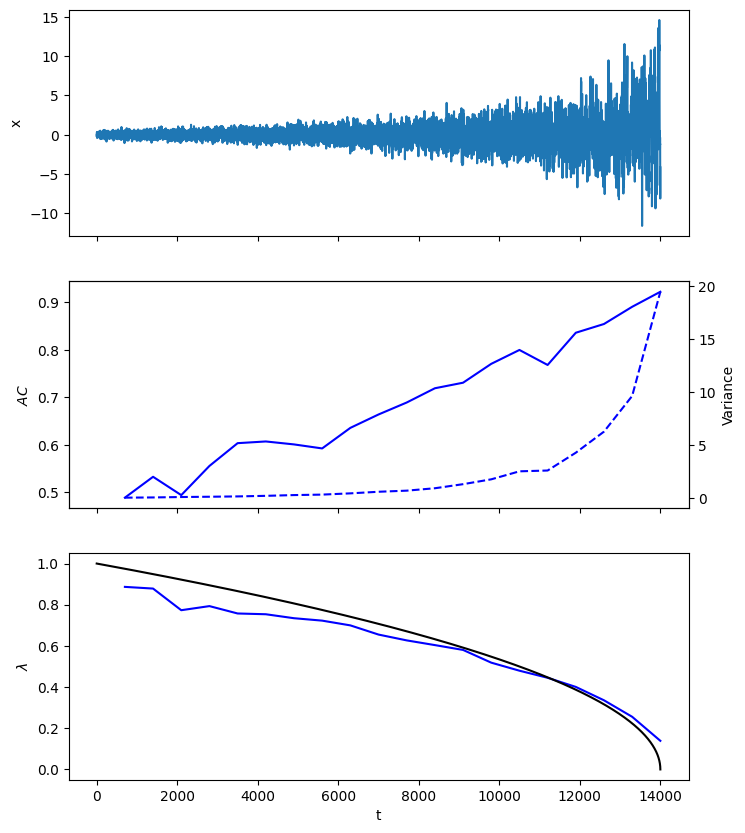
\includegraphics[width=\textwidth]{figures/true_positive.png}
    \end{minipage}
    \hfill
    \begin{minipage}{0.49\textwidth}
        \centering
        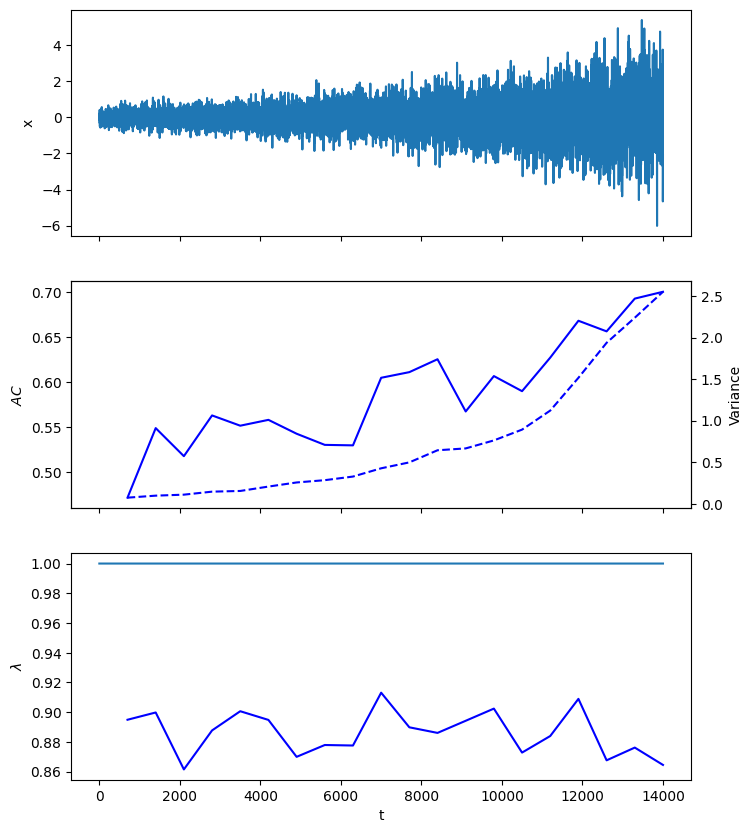
\includegraphics[width=\textwidth]{figures/false_positives.png}
    \end{minipage}
    \begin{minipage}{\textwidth}
    \centering
    \caption{Based on \cite{Morr:2024} Figure 1; AC: ---, Var: - - - \\
    We simulate two time series based on (\ref{failure of TEWS SDE}), where $(\kappa_{0},\kappa_{T},\theta_{0},\theta_{T}) = (1.2,3.3,3,1)$. In the left column there is CSD, which is captured by all indicators. The right column shows a false positive example for the TEWS methods, since $\lambda(t)$ is constant in this case. 
    }
    \label{false positive example}
    \end{minipage}
\end{figure}


Now we turn to a false negative example. For the simulation of both time series we choose: $(\kappa_{0},\kappa_{T},\theta_{0},\theta_{T}) = (3.2,2.3,1,3.7)$. In this case we have for decreasing $\lambda$ a decline in the variance beside the increase close to T and an increase in AC(1). Hence the variance gives a false negative signal. For fix $\lambda(t) \equiv \lambda_{0}$ both indicators a decreasing. This is again matched by the results from the simulation as seen in Figure \ref{false negative example}. The ROSA method again matches $\lambda(t)$ well and doesn't show false signals.

\begin{figure}
    \begin{minipage}{0.49\textwidth}
        \centering
        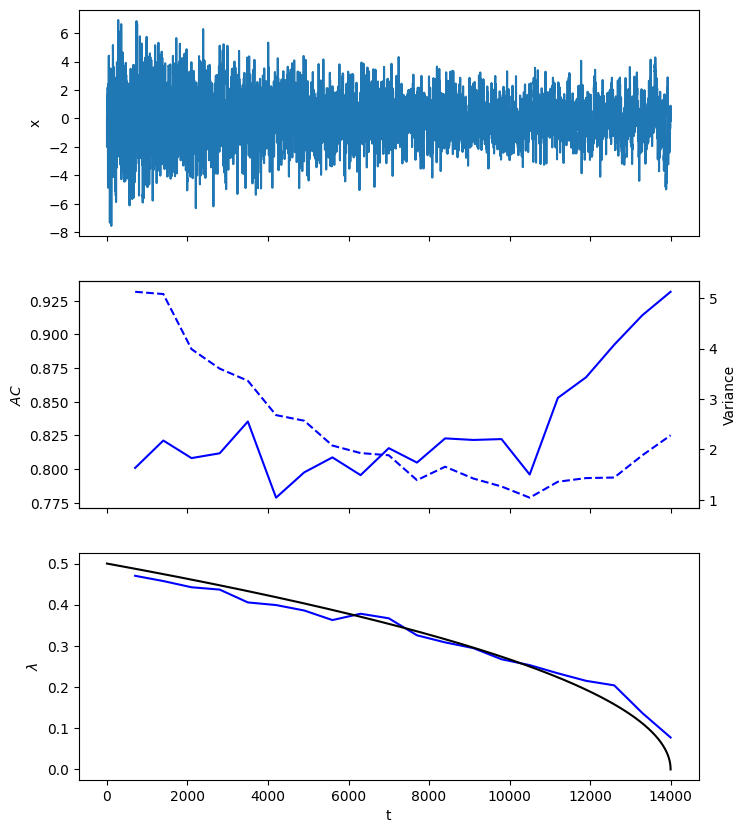
\includegraphics[width=\textwidth]{figures/false_negative_var.png}
    \end{minipage}
    \hfill
    \begin{minipage}{0.49\textwidth}
        \centering
        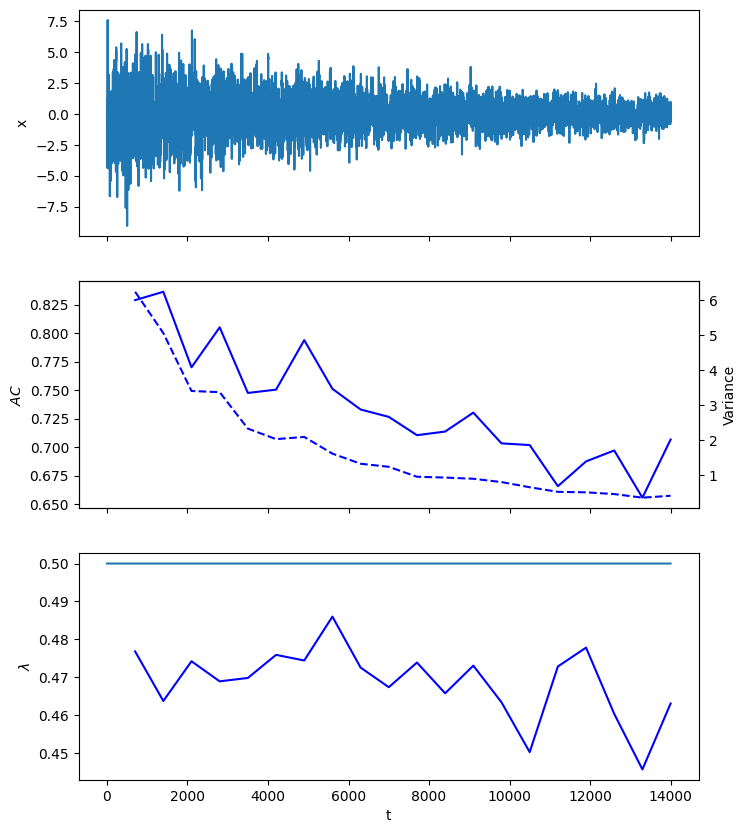
\includegraphics[width=\textwidth]{figures/true_negative.png}
    \end{minipage}
    \begin{minipage}{\textwidth}
    \centering
    \caption{Based on \cite{Morr:2024} Figure 3; AC: ---, Var: - - - \\
    We simulate two time series based on (\ref{failure of TEWS SDE}), where $(\kappa_{0},\kappa_{T},\theta_{0},\theta_{T}) = (3.2,2.3,1,3.7)$. In the left column, where $\lambda(t)$ is decreasing, the variance gives a false negative signal, while the ROSA method gives an EWS. In the right column, where $\lambda(t)$ is constant, no indicator gives an EWS. 
    }
    \label{false negative example}
    \end{minipage}    
\end{figure}


These were however only two examples. We want to provide more evidence for the robustness of the ROSA method, by comparing it to the old indicators on a wider ranch of parameter settings. This will be done in the next section.
    


\chapter{Benchmarking of traditional EWS with ROSA}

We showed the risk of false signals with the traditional EWS under changing parameters.
The ROSA method showed no wrong signals.
In this section we want to carry out a more thorough comparison in terms of false positives vs. true positives of the traditional EWS versus the ROSA method. We do this by plotting the ROC curve and computing the AUC values. First, we will do this for 100\% of observed CSD and then for 60\%.

We remind us of the test setting: 

\begin{subequations}
    \begin{align*}
        dX_{t} &= -\lambda(t) X_{t}dt + \kappa(t) U_{t}dt, X_{0} = 0 \\
        dU_{t} &= -\theta(t) U_{t}dt + dW_{t}, U_{0} = 0
    \end{align*}
\end{subequations}

Where $\lambda$ either decreases: 
    \[
    \lambda(t) := \lambda_{0}\sqrt{1-t/T}
    \]

Or stays fixed: 
    \[
    \lambda(t)\equiv\lambda_{0}
    \]

We want a reliable indicator, meaning one that leads to as few as possible false positives and as many as possible true positives. All indicators AC(1), Variance, and ROSA should show an increase in their indicator series for CSD. Hence we have to quantify what we define as a positive signal and what not. To do this we use the Kendall rank correlation coefficient (or Kendall's $\tau$ coefficient) as defined in \ref{def:Kendall tau} and choose a threshold above which we count something as a positive signal. 



The procedure to benchmark our indicators quantitatively is the following:
We generate n = 1000 parameter settings $(\lambda_{0},\kappa_{0},\kappa_{T},\theta_{0},\theta_{T})$ where $\lambda_{0} \sim \text{Unif}(0.3,0.5)$ and $\kappa_{0},\kappa_{T},\theta_{0},\theta_{T} \sim \text{Unif}(0.5,4)$. For each parameter setting we generate one time series where $\lambda(t)$ is decreasing and one where it is not, with a time span of T = 14000, window length of W = 700, $\delta t = 1/10$ and $\Delta t = 1$.


 We do this using the Euler Method. Then we compute the Variance, $AC(1)$, and ROSA indicators for both time series. Afterwards, we calculate the Kendall's $\tau$ value for the indicator series from the three EWS for decreasing and fixed evolution of $\lambda(t)$. We create an array of 1001 threshold values equally spaced between -1 and 1. To compute the true positive rate for all indicators we take the fraction of the corresponding Kendall's $\tau$ values of the 1000 settings with a decreasing $\lambda(t)$ that are greater than the threshold. We get the false positive rate in the same way, now only with the corresponding Kendall's $\tau$ values of the settings with a fixed $\lambda(t)$. This is repeated for all 1001 threshold values. We get the ROC curves by plotting the true positive rates against the false positive rates for the three indicators.
The AUC value is defined as the area under the ROC curve and can be computed from the false and true positive vectors. 

For a high threshold there is a high proportion of false negative signals for a decreasing $\lambda(t)$. When lowering the threshold for Kendall's $\tau$ from 1 to -1 (advancing from the bottom left corner to the top right in Figure (\ref{fig:ROC_curves})) we would like to have a fast increase in the true positive rate and a slow increase in the false positive rate. Hence a higher AUC value is better. In Figure (\ref{fig:ROC_curves}) we see that the ROSA method drastically outperforms the two traditional indicators. The $AC(1)$ method is better at detecting CSD than the variance.  
In the ROC curve plot we don't see the spacing of the threshold values. To gain the complete picture we allow for the whole range of Kendall's $\tau$ down to -1, hence counting negative trends as positive signals, which would be odd in practice. We mark the location of the threshold value 0 on the ROC curves. This is the lowest threshold for a reasonable indication of a true positive signal. Due to the symmetry of the trends for the null model, the corresponding false positive rate to this point is roughly 50\%. In practice we would choose a rather high threshold to increase the significance of positive results and to decrease the false positive rate.

For fold bifurcations a stark decline in the recovery rate shortly before the bifurcation is typical. However allowing the indicators in our test setup to observe the time series up until the time of tipping is problematic in two ways: it overestimates the usefulness of the indicator since in practice we want an indicator that warns us sufficiently early before tipping; also when approaching the tipping point noise-induced tipping, as described in Figure (\ref{fig:Critical transitions in the fold catastrophe mode}), can't be excluded \cite{Ashwin:2012,Meng:2020}. To assess the capability of the indicators to detect the approaching of a TP early enough, we perform the same analysis, but now only on 60\% of the data. The procedure stays the same, despite now calculating the indicators on only the first $12 = 20 \cdot 0.6$ windows. The ROC curve plots for both scenarios (100\% and 60\% of observed Data) are provided in Figure (\ref{fig:ROC_curves})


\begin{figure}[h!]
    \centering
    \begin{minipage}[t]{0.45\textwidth}
        \centering
        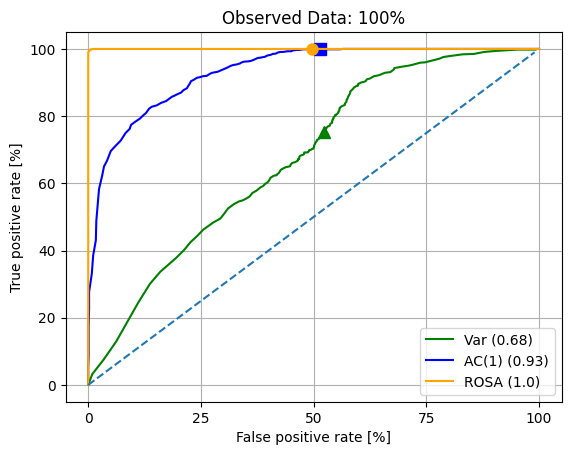
\includegraphics[width=\textwidth]{bachelor-thesis/figures/ROC_curves_100.png}
    \end{minipage}
    \hfill
    \begin{minipage}[t]{0.45\textwidth}
        \centering
        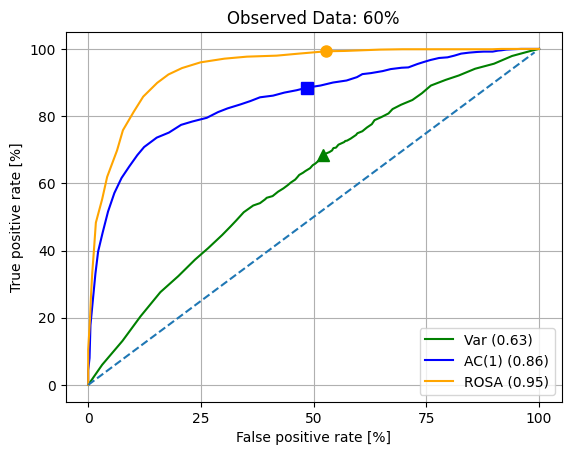
\includegraphics[width=\textwidth]{bachelor-thesis/figures/ROC_curves_60.png}
    \end{minipage}
    \vspace{0.5cm}
    
    % Add caption and label
    \caption{Based on \cite{Morr:2024}, Figure 2. In the left panel the analysis is conducted on the full evolution of $\lambda(t)$. For the AUC values, view the legend. The ROSA method shows perfect differentiation between false positives and true positives. The $AC(1)$ indicator is also significantly better than the variance. The location, where Kendall's $\tau$ is 0, is denoted by the symbols. In the right panel only 60\% of the data was observed. As expected all indicators performed in this case because the sharp decline of the recovery rate is not present in the data and hence the signs of CSD are more subtle. Again the ROSA method outperformed the traditional EWS with the $AC(1)$ being better than the variance.}
    \label{fig:ROC_curves}
\end{figure}
 

In \cite{Morr:2024} Morr described three additional indicators $\phi,\lambda^{(ACS)},\lambda^{(PSD)}$. In the case of 100\% observed data the AUC values were 0.99,1.0,1.0 (for $\phi,\lambda^{(ACS)},\lambda^{(PSD)}$ respectively) and in the case of 60\% of observed data it was 0.85,0.94,0.94 (for $\phi,\lambda^{(ACS)},\lambda^{(PSD)}$ respectively). We see that the ROSA indicator was at least as good as all of these in both cases.
The worse performance of the TEWS methods in the case of 60\% observed data is due to the fact, that changes in $\theta$ and $\kappa$ are now often relatively larger than the change in $\lambda(t)$, since the part of the sharp decline is missing now. This can mask the true evolution of $\lambda(t)$, as we have seen also in the previous section. The ROSA method performs worse because for cases of true CSD the Kendall $\tau$ value is smaller when only observing 60\% of the data since the sharp decline is not present. Hence the method detects fewer cases of true positives for a fixed threshold.

We want to further illustrate the dependence of quality of the indicators on the fraction of observed data and the length of the time series. For the dependence on the percentage of observed data we fix the time series length at T = 14000 and let the fractions vary in [0.2,0.4,0.6,0.8,1]. To analyze the dependence on the length of the time series, we fix the fraction of observed data at 60\% and let the time length vary in the range [5000,10000,15000,20000,25000,30000]. Figure \ref{fig:time_length_and_fraction_of_observed_data_dependence} shows that the quality of the traditional EWS methods mainly depend on the fraction of observed data, while the length of the time series is almost negligible. In contrast to that the power of the ROSA method increases both with a higher fraction of observed data as well as with a longer time series. The newly proposed method is again better than the old ones in all cases. 


\begin{figure}[h!]
    \centering
    \begin{minipage}[t]{0.45\textwidth}
        \centering
        \includegraphics[width=\textwidth]{bachelor-thesis/figures/fixed_length_vary_frac_500.png}
    \end{minipage}
    \hfill
    \begin{minipage}[t]{0.45\textwidth}
        \centering
        \includegraphics[width=\textwidth]{bachelor-thesis/figures/fixed_frac_vary_length_500.png}
    \end{minipage}
    \vspace{0.5cm}
    
    % Text below the figures
    \centering
    \begin{minipage}[b]{0.9\textwidth}
        \centering     
        Figure 9.2: 
    \end{minipage}
    \caption{Based on\cite{Morr:2024}, Figure 5. The left panel shows how the AUC values depend on the fraction of observed data for a fixed time series length of T = 14000. In the right panel the dependency of the AUC values on the time series length is displayed for a constant fraction of 60\% of observed data. }
    \label{fig:time_length_and_fraction_of_observed_data_dependence}
\end{figure}


\chapter{ROSA applied to the Snowball earth modell}

In this section we would like to apply the ROSA method to a climate model, where tipping occurs due to a fold-bifurcation: the Snowball Earth model, which is a simple Energy Balance Model (EBM). First, we shortly discuss the theory behind these simple models, taken from \cite{Kaper:2013}. The key quantity of Earth's climate system is temperature. In an EBM the state of Earth's climate is summarized in the variable temperature averaged over the entire globe. The simplest EBM doesn't cover any spatial dimensions and is thus sometimes referred to as zero-dimensional EBM. It is governed by an ODE. To derive this ODE we have to consider the energy budget of the Earth.

Almost all the energy for Earth's climate system comes from the sun in the form of electromagnetic radiation. A part of this is absorbed by the solar photosphere (the outer shell of a star). Treating the sun as a black body at 5780 K temperature is a good approximation for the solar energy spectrum.

The flux of solar radiation through a unit area of a sphere at a distance of one astronomical unit away from the sun is called the solar constant and is measured as $1,368Wm^{-2}$. Due to the sunspot cycle, it is not exactly constant but varies around $0.1\%$

The incident solar radiation (insolation) is more precise. It refers to the energy per unit area at a particular point in time and space. In contrast to the solar constant, the insolation varies significantly with time of day, season, latitude etc. To keep our model simple we stay with the solar constant.

When we neglect the differences among continents and oceans, in the composition of the atmosphere, topography, and other local features, we can characterize the state of the entire earth system by the single variable global mean surface temperature T. We want to know how T evolves over time. Though there are many complicated processes involved in determining T, we know that T will increase if the energy from the sun reaching Earth's surface exceeds the amount of energy emitted by Earth and vice versa.
The heat capacity of a system is the amount of energy needed to raise the temperature by one degree Celsius/Kelvin and is measured in Watt years per square meter [$W yr m^{-2}$]. For simplicity, we don't differentiate the heat capacity for different mediums and just consider it as the constant average value $C$ for the whole globe. If $A$ is the surface area of the earth and we have $T(t+\Delta t) = T(t) + \Delta T$, then we need $AC\Delta T$ energy to reach this new temperature.  Let $E_{in}$  ($E_{out}$) be the mean level of energy reaching (leaving) one square meter of the Earth's surface per unit time. Then we get: 
\begin{equation}
AC\Delta T = A(E_{in} - E_{out})\Delta t
\end{equation}
After canceling A, dividing by $\Delta t$, and letting it go to zero we get the following 0-dimensional EBM: 
\begin{equation}
    C\frac{dT}{dt} = E_{in} - E_{out}
\end{equation}
In an equilibrium we have $E_{in} = E_{out}$. Next, we want to find simple expressions for $E_{in}$ and $E_{out}$.

We start with a basic model.
Be $R$ the radius of the Earth and $S_{0}$ the solar constant. If we would look at the Earth from the sun it would appear as a flat disc with surface area $\pi R^2$. The Earth thus receives $\pi R^2 S_{0}$ solar energy per unit time. Only a fraction $1-\alpha$ of this reaches the surface, where $\alpha \in (0,1)$ is the sso-calledo called \textit{albedo} - the fraction reflected back to space. Locally the albedo differs drastically. Ice sheets for example reflect much more back than a desert does. For now we will again average the albedo over the entire globe. The energy $(1-\alpha)\pi R^2S_{0}$ is uniformly distributed over the Earth's surface area which is $4\pi R^2$. Hence the amount of Energy per square meter per unit time is $\frac{(1-\alpha)\pi R^2S_{0}}{(4\pi R^2)} = \frac{1}{4}(1-\alpha)S_{0}$. With $Q:=\frac{1}{4}S_{0}$ we get: 
\begin{equation}
    E_{in} = (1-\alpha)Q
\end{equation}
Now we consider $E_{out}$. The Earth also emits electromagnetic radiation, but mostly very long waves (infrared regime). We approximate the Earth as a black body with surface temperature $T$. Then according to the Stefan-Boltzmann law, the earth radiates 
\begin{equation}
    E_{out}(T) = \sigma T^4
\end{equation}
per unit area and per unit time, where $\sigma = 5.67 \cdot 10^{-8}Wm^{-2}K^{-4}$ is the Stefan's constant. In total we get: 
\begin{equation}
    C\frac{dT}{dt} = (1-\alpha)Q - \sigma T^4
    \label{temperature independent albedo EBM}
\end{equation}
Setting the right-hand side to zero we get the energy balance equation: 
\begin{equation}
    (1-\alpha)Q = \sigma T^4
\end{equation}
Solving for T: 
\begin{equation}
    T^* = (\frac{(1-\alpha)Q}{\sigma})^\frac{1}{4}
\end{equation}
With $Q = \frac{1}{4}S_{0}= 342 Wm^{-2}$ and $\alpha = 0.3$, which is a common value for Earth's albedo, we get an equilibrium temperature of $T^* = 254.8K$. This is much colder than our real surface temperature of $287.7K$. In the next paragraph we will include the greenhouse effect into our model, which can explain a large part of the difference.
\\ 
Greenhouse gases like carbon dioxide ($CO_{2}$), methane, water vapor, and aerosols (dust particles, water droplets, etc.) increase the opacity of the atmosphere in the infrared regime (wavelengths greater than $0.7 \mu m$). Due to the very different emitting temperatures of Earth and Sun, their emitting regimes barely intersect (Fig 2.4). While the sun emits only waves with lengths below $4 \mu m$ the earth emits only waves with lengths greater than $4 \mu m$. Hence the greenhouse effect decreases $E_{out}$ and has no impact on $E_{in}$. Therefore the global mean temperature increases. We incorporate this effect on $E_{out}$ by multiplying it with a factor $\epsilon \in (0,1)$. The modified energy balance equation: 
\begin{equation}
    (1-\alpha)Q = \epsilon \sigma T^4
\end{equation}
has the solution: 
\begin{equation}
    T^* = (\frac{(1-\alpha)Q}{\epsilon\sigma})^\frac{1}{4}
\end{equation}
We can get T* = 287.7K when we artificially choose $\epsilon = 0.62$, keeping $\alpha = 0.3$ and $S_{0} = 1,368 Wm^{-2}$. 
Now we want to improve our model further. 

A temperature-independent albedo does not account for the fact that snow and ice reflect sunlight much better than open water. We will include this observation in our simple model from (\ref{temperature independent albedo EBM}) by setting 
\begin{equation}
    \alpha (T) = 0.5 - 0.2 \cdot tanh(\frac{T - 265}{10})
\end{equation}
This gives us: 
\[
\alpha(T) =
\begin{cases}
0.7 & \text{if } T < 250K \\
0.3 & \text{if } T > 280K
\end{cases}
\]
This makes sure that a larger proportion of energy is reflected back to space when the temperature is low enough for the Earth to be covered by ice and snow.
The energy balance equation with a temperature-dependent $E_{in}$: 
\begin{equation}
 C\frac{dT}{dt} = (1-\alpha(T)Q - \epsilon\sigma T^4
 \label{simple EBM}
\end{equation}
Below we plot $(1-\alpha(T))Q$ and $\epsilon\sigma T^4$ against $T$. We see that there are three equilibria at $T_{1}^* = 288K$, $T_{2}^* = 265K$ and $T_{3}^* = 233K$, where $T_{1}^*$ and $T_{3}^*$ are stable and $T_{2}^*$ is unstable. Our current climate corresponds to $T_{1}^*$. In the \textit{Snowball Earth} scenario $T_{3}^*$ the earth would be entirely covered by snow and ice. 

\begin{figure}
    \centering
    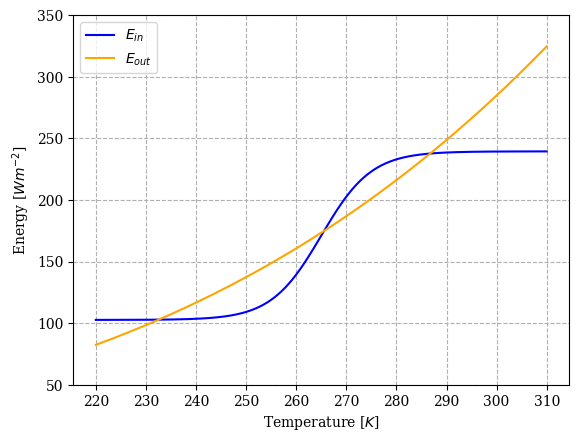
\includegraphics[width=0.7\textwidth]{bachelor-thesis/figures/se_multiple_equilibria.png}
    \caption{Based on \cite{Kaper:2013}, Figure 2.5. We plot $E_{in} = (1-\alpha(T))Q$ and $E_{out} = \epsilon\sigma T^4$ against T. There are three equilibria at $T_{1}^* = 288K$, $T_{2}^* = 265K$ and $T_{3}^* = 233K$.}
    \label{fig:enter-label}
\end{figure}

We have to keep in mind that the time scale of an EBM covers millions of years. Hence all recent ice ages and the most severe periods of glaciation of the last million years correspond to the state $T_{1}^*$. The question arises though, whether the planet has visited the state $T_{3}^*$ in the past. There is some geological evidence suggesting that the Earth was completely frozen during the Cryogenian (720-635 Myrs BP) and Huronian (2400 - 2100 Myrs BP) age (Lecture 2 Boers). How could the Earth escape this state of complete glaciation? There was still some CO2 released into the atmosphere e.g. from volcanic eruptions, but no biomass existed that could take this up. This lead to a large accumulation of CO2 and consequently an increase in the greenhouse effect. In our simple model this corresponds to a decrease of $\epsilon$ and the orange curve. At some point the stable equilibrium $T_{3}^*$ would vanish and the climate system would suddenly transition to a much warmer stable equilibrium. Paleoclimate records exist that provide evidence for such rapid change at the end of glaciation periods (Cambrian explosion). Other questions that come to mind are: why wasn't there a snowball earth period during the last 500 million years and could there be another one in the future? We know that the continents were closer to the equator during the Proterozoic age and that rock erosion is a main actor in the removal of CO2. This lead to a low level of CO2 and greenhouse gas effect, while the polar caps could expand during ice ages. With today's distribution of the continents being closer to the poles the rock erosion would end earlier during an ice age, leading to an earlier regulating effect due to the greenhouse gas effect. During the cold war there was the fear that an outbreak of a nuclear war could cause the earth to freeze. 

Now we want to understand how the equilibrium states develop when we change the solar constant $S_{0}$. To do this we plot the bifurcation diagram in Figure \ref{fig:se_bif}. We have a fold bifurcation model with bifurcation points at $Q_{-}$ and $Q_{+}$. Here $q := Q/Q_{0}$ is the bifurcation parameter, where $Q_{0} = 342 Wm^{-2}$. When we let $q$ cross $Q_{-}$ from above, then $T_{1}^*$ and $T_{2}^*$ merge and disappear, leading to the snowball earth state $T_{3}^*$ (lower branch). If we cross $Q_{+}$ from below, then we only have the state $T_{1}^*$ (upper branch) free of ice. 

In the next step we want to apply the traditional EWS and the ROSA method to our simple EBM.
The simulation works the same as described in earlier sections only now with a different function used for the SDE. We let our time series start in the lower branch and linearly increase $q$ until the time series tips over into the upper branch. In the upper panel of fig \ref{fig:ROSA tes} we see the full picture, where $q$ ranges from 0.7 to 1.4. We observe that the rate $\lambda(t)$ first increases before going to zero. In the previous sections we always had the case that we computed our EWS methods only on the already decreasing part of $\lambda$. As we see here this doesn't have to be the case in general. To better compare our methods we simulate the time series again in the more crucial region of $q \in [1.1,1.3]$ as illustrated in the lower row of Figure \ref{fig:ROSA test}. In the left panel the system is driven by white noise and all methods show an increase as expected. The Kendall $\tau$ coefficients are given by 0.47 (AC(1)), 0.73 (Variance), 0.86 $(-\widehat{\lambda})$. In the right panel we provoke a false negative for the traditional EWS by linearly decreasing $\kappa$ (from 3.2 to 2.3) and linearly increasing $\theta$ (from 1 to 3.7). The ROSA method also works in the red noise case.

\begin{figure}[t]
    \centering
    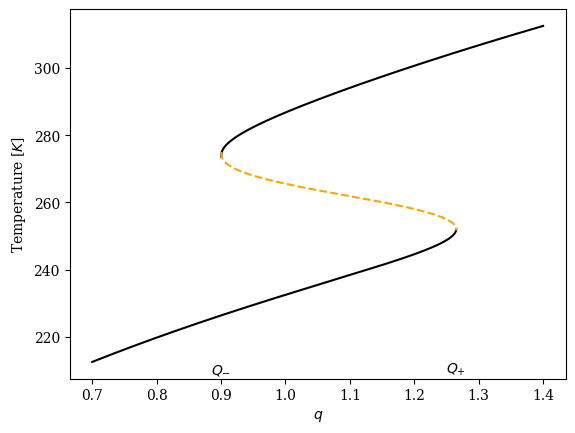
\includegraphics[width=0.6\textwidth]{bachelor-thesis/figures/se_bif_plot.png}
    \caption{Based on \cite{Kaper:2013}, Figure 2.6. Here we show the dependency of the equilibrium states on the bifurcation parameter $q = Q/Q_{0}$. We observe that the system (\ref{simple EBM}) exhibits a fold bifurcation.   }
    \label{fig:se_bif}
\end{figure}



\begin{figure}[b]
    \centering
    \includegraphics[width=0.9\textwidth]{bachelor-thesis/figures/11_9_se_ROSA.png}
    \caption{We apply our three indicators to the simple EBM as defined in (\ref{simple EBM}) driven by red noise. In the upper row the bifurcation parameter ranges from 0.7 to 1.4  and in the lower row from 1.1 to 1.3. We use $(\kappa_{0},\kappa_{T},\theta_{0},\theta_{T}) = (1,1,1,1)$ in the upper and lower left panel and $(\kappa_{0},\kappa_{T},\theta_{0},\theta_{T}) = (3.2,2.3,1,3.7)$ in the lower right panel, where we observe a false negative signal by the Variance method.}
    \label{fig:ROSA test}
\end{figure}



\appendix
\chapter{Appendix}
The code generating the figures in this thesis can be accessed at the following GitHub repository: \\
https://github.com/j-dichgans/Code-for-Bachelor-Thesis/tree/master


\backmatter{}
\listoffigures% may be removed
\listoftables% may be removed

\nocite{Alspach:2008,GaleShapley:1962} % further literature that has not been explicitly referenced in the text
\printbibliography{} % print bibliography

\end{document}

%%% Local Variables:
%%% mode: latex
%%% TeX-engine: default
%%% TeX-command-extra-options: "-shell-escape"
%%% ispell-local-dictionary: "american"
%%% eval: (setenv "TEXINPUTS" ".//:")
%%% TeX-master: t
%%% End:
